%====================================================================================
% Preamble
%------------------------------------------------------------------------------------

\documentclass{beamer}

% Essential Packages
% Apartado de letras
\usepackage[utf8]{inputenc}
\usepackage[T1]{fontenc}
\usepackage[spanish]{babel}

% Aparatdo matemático
\usepackage{amsmath}
\usepackage{amsfonts}
\usepackage{amssymb}
\usepackage{mathtools}

% Apartado tablas, figuras, y otros
\usepackage{multirow,booktabs,setspace,caption,multicol,tabularx, tabulary}
\captionsetup{skip=0pt}

% Apartado Tablas y Figuras en APA
\DeclareCaptionLabelSeparator*{spaced}{\\[1ex]}
\captionsetup[table]{name = Tabla, textfont=it,format=plain,justification=justified,
	singlelinecheck=false,labelsep=spaced,skip=0pt}
\captionsetup[figure]{name = Figura, labelsep=period,labelfont=it,justification=justified,
	singlelinecheck=false,font=doublespacing}
	% Para hacer tablas APA más fácil
	\usepackage[flushleft]{threeparttable}

% Apartado hyperres
\usepackage{hyperref}

% Apartado Tikz
\usepackage{tikz, pgfplots}
\usetikzlibrary{positioning,calc,arrows}
\usetikzlibrary{shapes.arrows}
\usetikzlibrary{patterns}

	\tikzset{ % to make dots on the graph
		dot/.style = {circle, fill, minimum size=#1,
			inner sep=0pt, outer sep=0pt},
		dot/.default = 6pt % size of the circle diameter 
	}

% Apartado de colores
\usepackage{xcolor}

% Apartado tipò de letra
\usepackage{textcomp}
\usepackage{libertine}
\usepackage[libertine]{newtxmath}

% Apartado de íconos
\usepackage{fontawesome5}

%Creación de entornos matemáticas
\newtheorem{defi}{Definición}[section]
\newtheorem{lema}{Lema}[section]
\newtheorem{teo}{Teorema}[section]
\newtheorem{coro}{Corolario}[section]

% Diversos
\usefonttheme[onlymath]{serif}
\usepackage{remreset}
\usepackage{makecell}
\usepackage{float}
\usepackage{subfigure}

% Apartado justificación de textos
\usepackage{ragged2e}
\justifying
\renewcommand{\raggedright}{\leftskip=0pt \rightskip=0pt plus 0cm}

% Apartado de configuración del Beamer
\mode<presentation> {
	\usetheme{Frankfurt}
	\setbeameroption{show notes}
	\setbeamertemplate{footline}[frame number]
	\usefonttheme[onlylarge]{structuresmallcapsserif}
	\usefonttheme[onlysmall]{structurebold}
	\usecolortheme{beaver}
	\setbeamercovered{transparent}
	\setbeamertemplate{navigation symbols}{}
	
	\setbeamercolor{section in head/foot}{bg=gray!8!white,fg=yellow!25!red}	
	\setbeamercolor{frametitle}{bg=gray!15!white,fg=yellow!20!red}
	\setbeamercolor{title}{bg=gray!25!white,fg=yellow!20!red}
	\setbeamercolor{item projected}{fg=white,bg=yellow!30!red}
}

% Apartado transparencia de contenido
\AtBeginSection[]
{
	\begin{frame}<beamer>{Contenido}
		\tableofcontents[currentsection,currentsubsection]
	\end{frame}
}
\AtBeginSubsection[]
{
	\begin{frame}<beamer>{Contenido}
		\tableofcontents[currentsection,currentsubsection]
	\end{frame}
}

% Apartado de logo
\logo{
\includegraphics[scale=.12]{figures/logo.png}}

% Apartado cambio como por punto
\decimalpoint

%====================================================================================

%====================================================================================
% Body
%====================================================================================
% Title Page
%-----------
\title{Teoría Microeconómica II\\
		Tema 1: COMPLETAR}
\author[José A. Valderrama]{\large{José A. Valderrama}\\
		{\small \texttt{jvalder@ulima.edu.pe} {\color{black}{\faIcon{envelope}}}}}
\institute{\large Universidad de Lima - Carrera de Economía}

\date{\today}

%------------------------------------------------------------------------------------
% Title
%---------
\begin{document}
	\begin{frame}[plain]
		\maketitle
	\end{frame}
%------------------------------------------------------------------------------------
% Sections
%---------
	\begin{frame}{Contenido}
		\tableofcontents
	\end{frame}

%1) Intercambio puro ----------------------------
	%====================================================================================
\section{Introducción}
%====================================================================================

\begin{frame}{Introducción}
	La selección adversa es un problema en que las partes contratantes no se conocen a la perfección.\\[0.3cm]
	
	Aparece cuando el agente tiene más información sobre alguna de las variables relevantes para la relación\\[0.3cm]
	
	Quien posee ventaja informativa sobre un tercero puede tener interés para ocultarla o usarla para su propio beneficio\\[0.3cm]
	
	Consecuencias:
		\begin{itemize}
			\item modificaciones en el equilibrio de mercado
			\item Inexistencia de equilibrio.
		\end{itemize}
\end{frame}
%2) Caja de Edgeworth ---------------------------
	%====================================================================================
\section[Akerlof]{El mercado de autos usados (artículo de Akerlof}
%====================================================================================

\begin{frame}{El artículo de Akerlof}
	Fue el primero que introdujo el concepto de información asimétrica\\[0.3cm]
	Su argumento básico es que en muchos mercados el comprador emplea alguna estadística del mercado para medir el valor de una clase de bienes\\[0.3cm]
	Entonces , el comprador mira el promedio del mercado completo mientras el vendedor tiene más conocimiento privado de un aspecto específico\\[0.3cm]
	Según Akerlof esta información asimétrica le da al vendedor un incentivo para vender bienes por debajo de la calidad media del mercado\\[0.3cm]
	
\end{frame}
%------------------------------------------------
\begin{frame}{El artículo de Akerlof}
	Entonces , la calidad promedio de los bienes en el mercado se reducirá con el tamaño del mercado\\[0.3cm]
	Tales diferencias en retornos sociales y privados puede ser mitigado por un número de diferentes instituciones del mercado\\[0.3cm]
	Akerlof empieza asumiendo un modelo del mercado de automóviles , donde hay cuatro tipos de autos:
		\begin{itemize}
			\item Hay autos nuevos y autos viejos ,
			\item En cada uno , pueden ser autos buenos o malos
			\item Los autos malos son popularmente conocidos como ``limones'' en EEUU.
		\end{itemize}

\end{frame}
%------------------------------------------------
\begin{frame}{El artículo de Akerlof}
	Existen dos tipos de agentes: Compradores y Vendedores
		\begin{enumerate}
			\item Compradores
				\begin{itemize}
					\item Función de utilidad: $U_v = M +1.5qn$
						\begin{itemize}
							\item $M$ = Consumo de otros bienes
							\item $q$ = Calidad del auto
							\item $n$ = $\left\lbrace 0,1\right\rbrace $ 1 compra auto, 0 no compra
						\end{itemize}
					\item Restricción presupuestaria: $y_v = M + pn$
						\begin{itemize}
							\item $y_c$ = Ingreso
							\item $p$ = Precio del auto
						\end{itemize}
				\end{itemize}
			La calidad del auto $(q)$ es información privada del vendedor. El comprador aprecia $``q''$ como la calidad media del mercado, mientras que el vendedor distingue la de cada auto
		\end{enumerate}
\end{frame}
%------------------------------------------------
\begin{frame}{El artículo de Akerlof}
	Dada la incertidumbre de $``q''$ el comprador maximiza su utilidad esperada:
		\begin{itemize}
			\item $E(U_c)=M+1.5E(q)n \quad E(q) = \mu =$ Calidad media observada
		\end{itemize}
	Sustituyendo $M$ de la $r.p .$ $\longrightarrow M =y_c - pn$ 
		\begin{itemize}
			\item $E(U_c) = y_c - pn + 1.5\mu n \longrightarrow $  factor común a ``$n$''
			\item $E[U_c] = y_c +\left[ 1.5\mu - p\right]n$
		\end{itemize}
	Decisión:
		\begin{itemize}
			\item $n=1$ compra si percibe la calidad del auto por encima del precio; es decir, si $1.5\mu \geq p$
			\item $n=0$ no compra si percibe la calidad del auto por encima del precio; es decir, si $1.5\mu \leq p$
		\end{itemize}
\end{frame}
%------------------------------------------------
\begin{frame}{El artículo de Akerlof}
	\begin{enumerate}[2]
		\item Vendedores
			\begin{itemize}
				\item Función de utilidad:$U_v = M +qn$
				\item Restricción presupuestaria: $y_v = M + pn$
				\item $n=1$ mantener el auto, $n=0$ vender del auto
			\end{itemize}
		Por tanto:
			\begin{itemize}
				\item Para el vendedor la $U_{MG} = q$
				\item Para el comprador la $U_{MG} = 1.5q$
			\end{itemize}
		Esto es lo que garantiza potenciales ganancias en el intercambio.
	\end{enumerate}
\end{frame}
%------------------------------------------------
\begin{frame}{El artículo de Akerlof}
	El vendedor conoce $q$
		\begin{itemize}
			\item Sustituyendo $M$ de la $r.p.$ donde $M=y_v - pn$
			\item $U_v = y_v - pn +qn \longrightarrow $factor común a ``$n$''
			\item $U_v = y_v + (q-p)n$
		\end{itemize}
	Decisión
		\begin{itemize}
			\item $n = 0$ vende si $p\geq p$ (Precios $\geq$ Calidad)
			\item $n = $ vende si $p\leq p$ (Precios $\leq$ Calidad)
		\end{itemize}
	¿Cómo se forma $\mu$
\end{frame}
%------------------------------------------------
\begin{frame}{El artículo de Akerlof}
	Akerlof partió del supuesto simplificador que la calidad de los autos se distribuye de manera uniforme en el rango $[0,2]$, por tanto $f(q)= 1/2$\\[0.3cm]
	
	La oferta de autos es $S=(1/2)pN$ porque:
		\begin{itemize}
			\item la probabilidad de vender es $(1/2)p$
			\item Número de autos usados $()N$
		\end{itemize}
	Es decir, la oferta es el número de autos usados por la probabilidad de venta. Tenemos todos los datos necesarios para calcular el equilibrio de esta economía
		\begin{itemize}
			\item Demanda: $(3/2) \mu \geq p$
			\item Oferta:$(1/2)pN$
			\item Calidad media: $(1/2)p$
		\end{itemize}
	Con lo que no existe ningún precio que cumpla las condiciones
		\begin{itemize}
			\item Demanda: $(3/2) \mu \geq p \rightarrow \mu=(1/2)p \rightarrow (3/2)(1/2)p\geq p \rightarrow (3/4)p\geq p \rightarrow $ \textbf{CONTRADICCIÓN}
		\end{itemize}
\end{frame}
%------------------------------------------------
\begin{frame}{El artículo de Akerlof}
Existe el colapso total del mercado y la única diferencia de este modelo con uno convencional de competencia perfecta es la asimetría de la información. Este modelo es ineficiente en el sentido de Pareto debido a la estructura de la información.\\[0.3cm]
El colapso total del mercado es consecuencia en parte de la parametrizacion del modelo. Es posible determinar una valoración marginal del comprador para que se produzca el intercambio.
\end{frame}
%------------------------------------------------
\begin{frame}{El artículo de Akerlof}
	\begin{itemize}
		\item Utilidad del comprador $\longrightarrow U_c = M+\beta qn$
		\item Regla de compra $\longrightarrow \beta \mu \geq p$
		\item La calidad de los autos se distribuye uniformemente $\mu = (1/2)p$
		\item Sustituimos $\mu$ en la regla de compra $\longrightarrow \beta(1/2)p \geq p$
		\item Por tanto $\beta \geq 2$ y lograría un precio bajo y como consecuencia el intercambio.
		\item Si la valoración del auto es alta, el comprador se arriesgará a pesar de la alta presencia de limones.
	\end{itemize}
\end{frame}
%------------------------------------------------
\begin{frame}{El artículo de Akerlof}
	El intercambio dejaría de existir produciendo el colapso del mercado a pesar de habría vendedores dispuesto a intercambiar el auto al precio ``$p$'' y compradores a adquirirlo.\\[0.3cm]
	Pero la información asimétrica impide que se realicen intercambios beneficiosos para ambas partes.
\end{frame}
%------------------------------------------------
\begin{frame}{Ejemplo}
	Seguros:
		\begin{itemize}
			\item Las personas mayores de 65 años casi no pueden comprar un seguro médico, incluso si están dispuestos a pagar un alto precio. Las compañías de seguros saben que con un precio alto, solo aquellos que tienen más probabilidades de aprovechar el seguro comprarán la póliza. Por lo tanto, las pólizas rara vez se venden en este mercado en particular.
		\end{itemize}
\end{frame}
%------------------------------------------------
\begin{frame}{Ejemplo}
	Costo de deshonestidad
		\begin{itemize}
			\item La presencia de personas que venden productos inferiores tiende a expulsar el negocio legítimo. No solo los consumidores son engañados, sino que también aumentan las preocupaciones morales y legales.
			
			\item La experiencia para decir el verdadero valor de los bienes no distinguibles se dirige fácilmente al arbitraje en lugar del propósito de producción real porque el primero es más rentable en un mundo lleno de limones.
		\end{itemize}
\end{frame}
%------------------------------------------------
\begin{frame}{Ejemplo}
	Mercado crediticio en países en desarrollo
		\begin{itemize}
			\item Los empresarios tienen que recurrir a ``agencias gestoras'', personas y empresas con reputación e influencia comunitaria, para financiar a una empresa recién creada.
			\item El mercado de crédito rural está dominado por préstamos con tasas exorbitantes de prestamistas locales en lugar de aquellos con tasas oficiales de bancos formales, ya que solo los primeros tienen buen acceso a la información del prestatario. Cualquiera que intente arbitraje tiende a perder.
		\end{itemize}
\end{frame}
%3) Curva de contrato  --------------------------
	%====================================================================================
\section[Producción]{Externalidades de producción}
%====================================================================================

\begin{frame}{Externalidades de producción}
Se definen:
	\begin{itemize}
		\item Costo Marginal Privado $(CMgP)$ o Costo marginal $(CMg)$ = costo de los factores de producción.
		\item Externalidad $(Ext)$ o Costo Externo marginal $(CEMg)$ = aumento del costo impuesto externamente cuando una o más empresas aumentan su producción en una unidad.
		\item Costo Marginal Social $(CMgS)$ o Costo Social marginal $(CSMg)= CMg + CEMg$.
	\end{itemize}
\end{frame}
%------------------------------------------------
\begin{frame}{Externalidades de producción}
		\begin{center}
		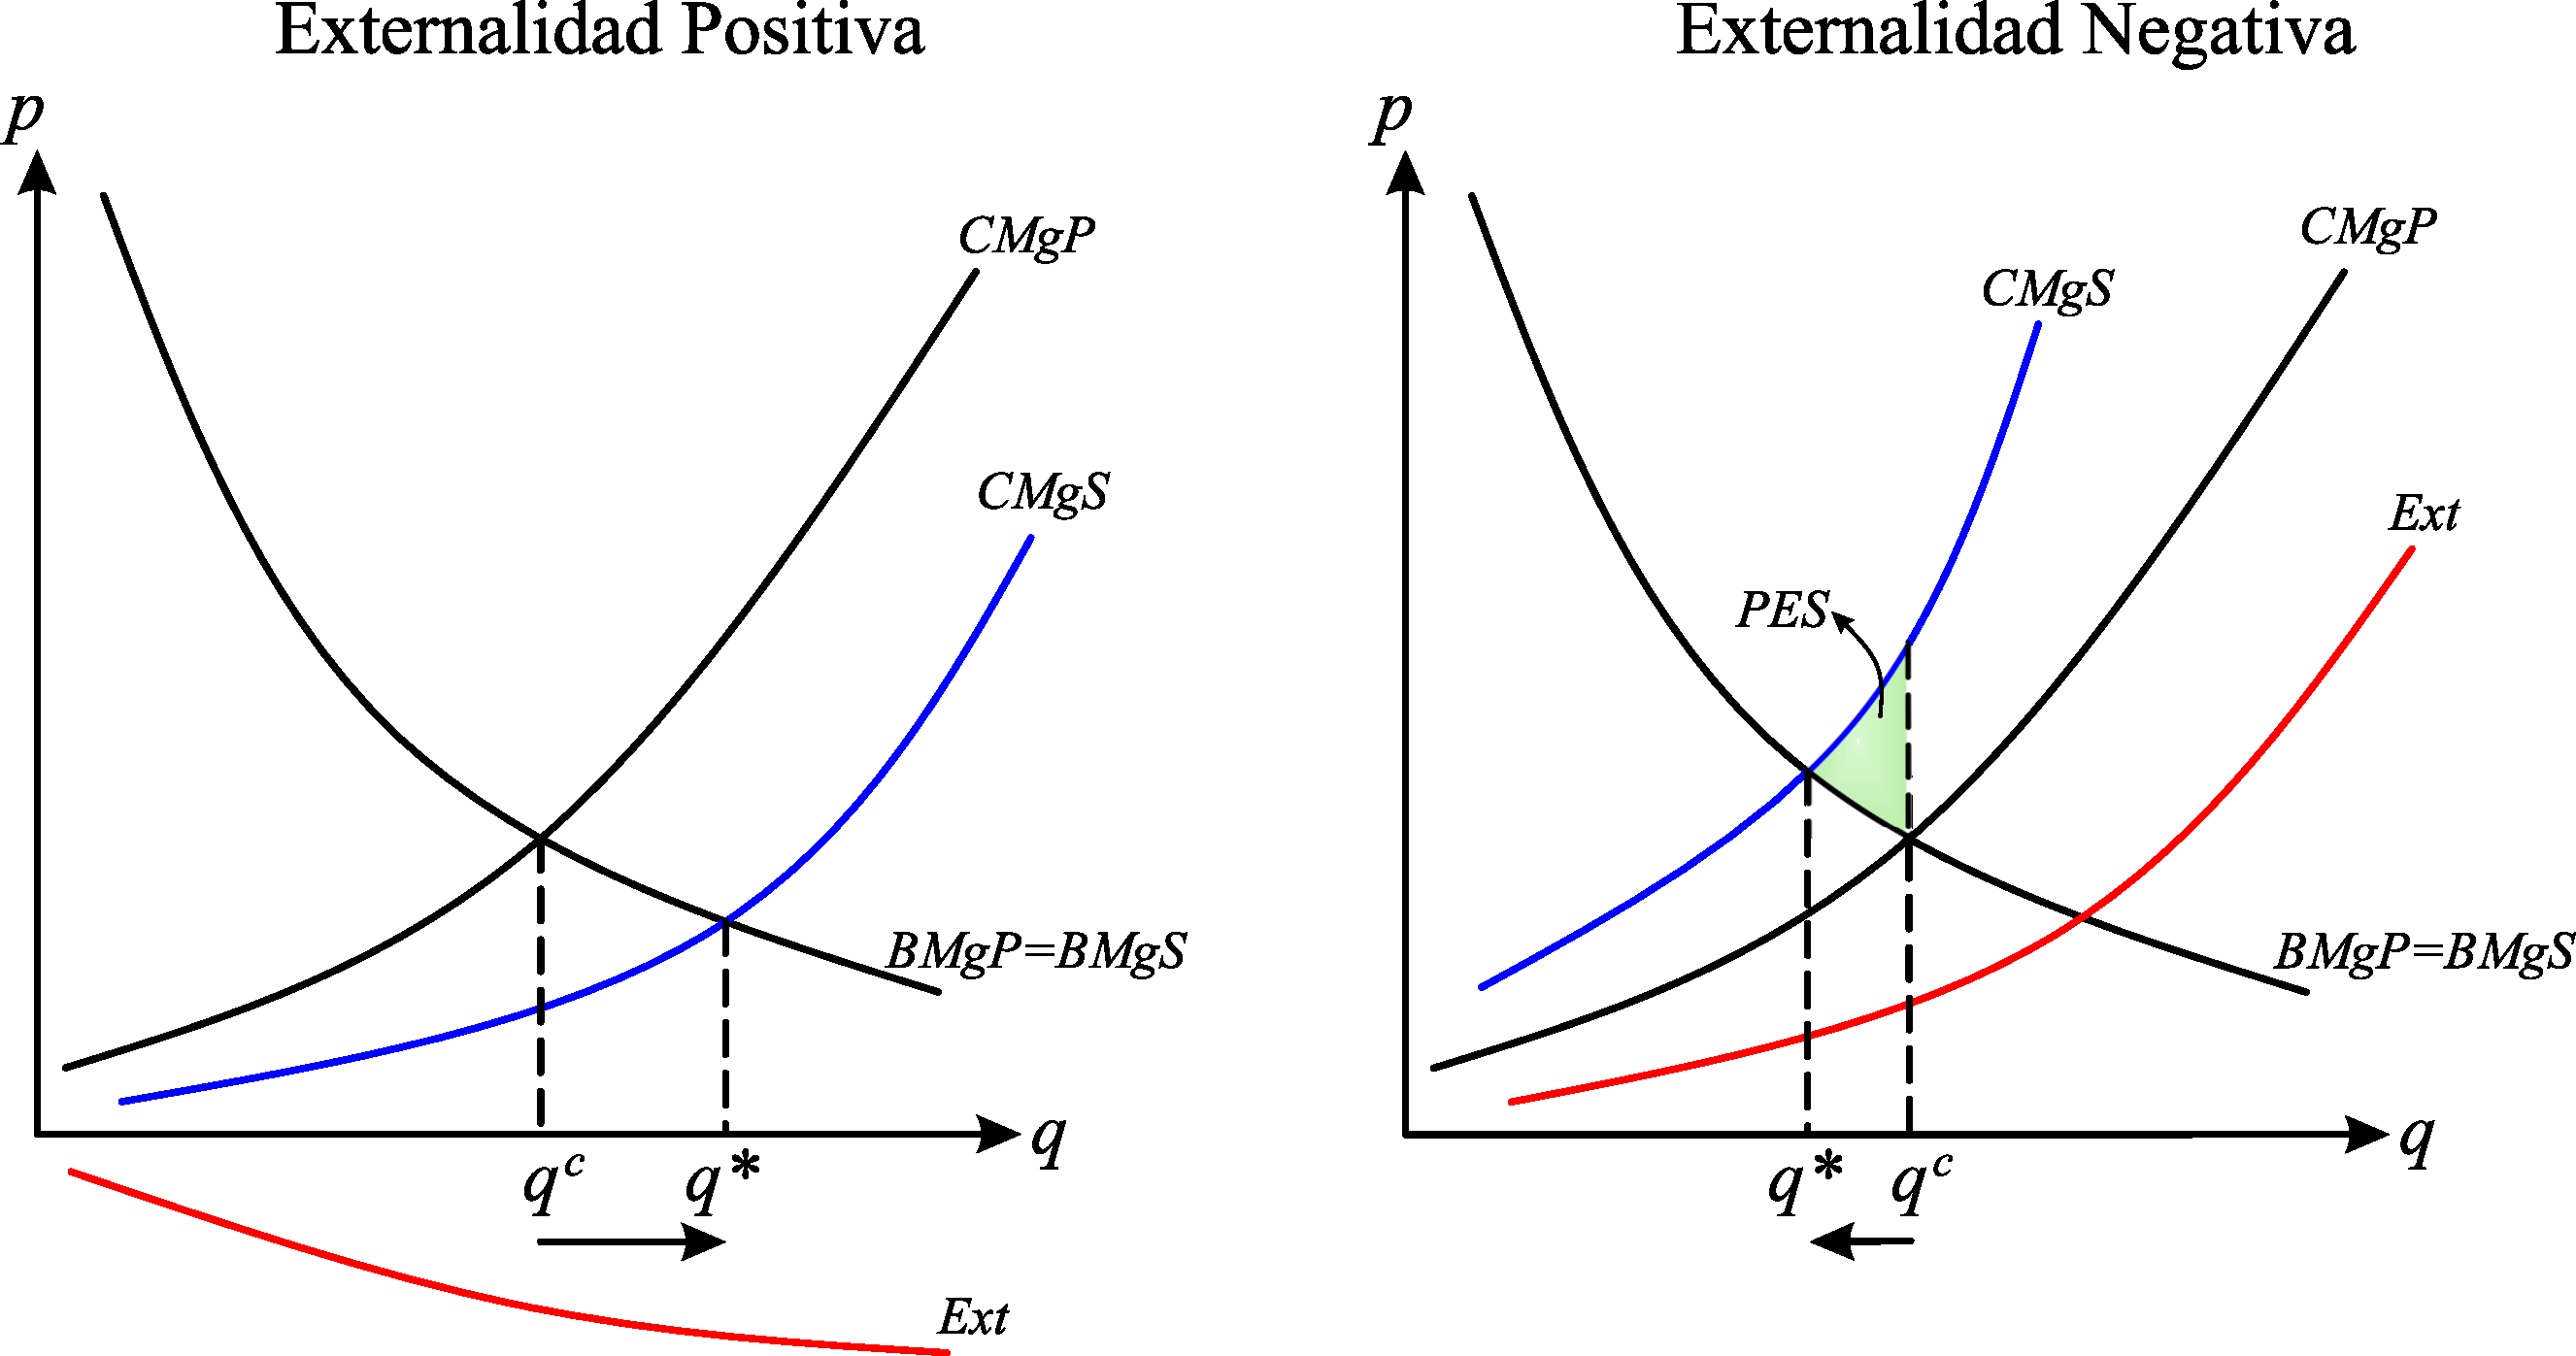
\includegraphics[width = 1\linewidth]{figures/produccion.pdf}
	\end{center}
\end{frame}
%------------------------------------------------
\begin{frame}{Externalidades de producción}
	\begin{itemize}
		\item Sean dos empresas: una acería $(S)$ y una piscigranja $(F)$.
		\item La empresa $S$ produce
			\begin{itemize}
				\item $s$ cantidad de acero
				\item $x$ cantidad de contaminación que se vierte a un río contiguo.
			\end{itemize}
		\item La empresa $F$ produce
			\begin{itemize}
				\item $f$ cantidad de pescado
			\end{itemize}
		\item La empresa $F$ se encuentra río abajo y se perjudica por la contaminación de la empresa $S$.
		\item Las funciones de costo son:
			\begin{itemize}
				\item Para S: $c_s(s,x)$
				\item Para F: $c_f(f,x)$
			\end{itemize}
	\end{itemize}
\end{frame}
%------------------------------------------------
\begin{frame}{Externalidades de producción}
	Supuestos
		\begin{itemize}
			\item La mayor contaminación eleva el costo de la producción de pescado
					$$\frac{\partial c_f}{\partial x} > 0$$
			\item La reducción del nivel de contaminación, elevará el costo de producción de acero
					$$\frac{\partial c_s}{\partial x} \leq 0$$
		\end{itemize}
\end{frame}
%------------------------------------------------
\begin{frame}{Problemas de maximización de beneficio}
	\begin{itemize}
		\item Para la acería: 
				$$\M \limits_{s,x} \pi_s = p_ss - c_s(s,x)$$
			  La acería elige la producción de acero y de contaminación que maximice su $\pi$.
		\item Para la piscigranja: 
				$$\M \limits_{f}\pi_f = p_f - c_f(f,x)$$
		      La piscigranja sólo determina cantidad de pescado, no controla la contaminación.
	\end{itemize}
\end{frame}
%------------------------------------------------
\begin{frame}{Problemas de maximización de beneficio}
	\begingroup
		\setlength{\tabcolsep}{10pt} % Default value: 6pt
		\renewcommand{\arraystretch}{1.5} % Default value: 1
			\begin{tabular}{ccc}
				\hline
					Para la acería & {} & Para la piscigranja\\
					$\M \limits_{s,x} \pi_s = p_ss - c_s(s,x)$ & {} & $\M \limits_{f} \pi_f = p_f - c_f(f,x)$\\
				\hline 
					\multicolumn{3}{c}{condiciones de primer orden} \\
				\hline
					$\frac{\partial \pi}{\partial s} = 0 \Leftrightarrow p_s - \frac{\partial c_s(s^\ast,x^\ast)}{\partial s} = 0$ & {} & $\frac{\partial \pi}{\partial f} = 0 \Leftrightarrow p_f - \frac{\partial c_f(f^\ast,x^\ast)}{\partial f} = 0$\\
					$p_s = \frac{\partial c_s(s^\ast,x^\ast)}{\partial s}$ & {} & $p_f = \frac{\partial c_f(f^\ast,x^\ast)}{\partial f}$\\
					$\frac{\partial \pi}{\partial x} = 0 \Leftrightarrow - \frac{\partial c_s(s^\ast,x^\ast)}{\partial x} = 0$ &{} & {}\\
					$0 = \frac{\partial c_s(s^\ast,x^\ast)}{\partial x}$& {} & {} \\
				\hline
			\end{tabular}
	\endgroup
\end{frame}
%------------------------------------------------
\begin{frame}{Problemas de maximización de beneficio}
	Interpretación
		\begin{itemize}
			\item La acería produce acero donde precio = $CMg$ de producir dicho acero.
					$$p_s = \frac{\partial c_s(s^\ast,x^\ast)}{\partial s}$$
			\item Y genera desechos donde el $CMg$ de producirlos es nulo.
					$$0 = \frac{\partial c_s(s^\ast,x^\ast)}{\partial x}$$
			\item La piscifactoría produce donde precio de pescado = CMg de producir pescado.
					$$p_f = \frac{\partial c_f(f^\ast,x^\ast)}{\partial f}$$
		\end{itemize}
\end{frame}
%------------------------------------------------
\begin{frame}{¿Por qué hay externalidad?}
	\begin{itemize}
		\item La acería produce demasiada contaminación, porque no le cuesta hacerlo.
		\item La cantidad óptima de acero sólo considera su costo de producción, no el daño que ocasiona a la piscigranja. 
		\item Como la piscigranja no puede controlar la cantidad de desecho que genera la acería, debe incurrir en mayores costos para eliminar el desecho del agua.
	\end{itemize}
\end{frame}
%------------------------------------------------
\begin{frame}{La solución eficiente}
	Fusionarse y maximizar el beneficio conjunto:
			$$\pi_s + \pi_f = p_ss - c_s(s,x) + p_ff - c_f(f,x)$$
				\vspace{-0.4cm}
		\begin{itemize}
			\item La empresa conjunta tiene en cuenta ahora los costos de todos los agentes ( costos de la producción de acero +  daño que le produce a la piscicultura). 
			\item Si: 
					$$\pi = p_ss + p_ff - c_s(s,x) - c_f(f,x)$$
			\item Las CPO son:
					\begin{gather*}
						\frac{\partial \pi}{\partial s} = 0 \Leftrightarrow p_s - \frac{\partial c_s(s^\ast,x^\ast)}{\partial s} = 0 \Leftrightarrow p_s - \frac{\partial c_S}{\partial s} - \frac{\partial c_f}{\partial x} \cdot \frac{\partial x}{\partial s} = 0\\
						p_s =  \frac{\partial c_s}{\partial s} + \frac{\partial c_f}{\partial x} \cdot \frac{\partial x}{\partial s}
					\end{gather*}
		\end{itemize}
\end{frame}
%------------------------------------------------
\begin{frame}{Gráficamente}
Por tanto, la producción óptima social de acero será menor a la producción privada.
	\begin{center}
		\begin{tikzpicture}[scale=1]
	% Formación de la caja
	% Consumidor A
	\draw[->] (0.5,0.5) node[align=center, below left] {\footnotesize $O_A$} -- (0.5,4.5) node[align=center, above] {\footnotesize $x_{2}^{A}$};
	\draw[->] (0.5,0.5) -- (8.5,0.5) node[align=center, right] {\footnotesize $x_{1}^{A}$};
	
	\draw (6,0.5) node[below] {\footnotesize $x_{1}^{A}$};
	\draw (0.5,2) node[left] {\footnotesize $x_{2}^{A}$};
	
	% Llaves
	\draw [decorate,decoration={brace,amplitude=5pt},xshift=-4pt,yshift=0pt] (6.1,-0.05) -- (0.7,-0.05);
	\node [right] at (3,-0.4) {$w_{1}^{A}$};
	
	\draw [decorate,decoration={brace,amplitude=5pt},xshift=-4pt,yshift=0pt] (-0.05,0.5) --(-0.05,2);
	\node [left] at (-0.3,1.27) {$w_{2}^{A}$};
\end{tikzpicture}
	\end{center}
\end{frame}
%------------------------------------------------
\begin{frame}{La solución eficiente}
	\begin{center}
		\begingroup
		\setlength{\tabcolsep}{10pt} % Default value: 6pt
		\renewcommand{\arraystretch}{1.5} % Default value: 1
			\begin{tabular}{p{4cm}cp{4cm}}
				\hline
					\multicolumn{3}{c}{Si: $\pi= p_ss + p_ff - c_s(s,x) - c_f(f,x)$} \\
				\hline
					Las CPO son: &{}&\\
				\hline
					$\frac{\partial \pi}{\partial x} = 0 \Leftrightarrow -\frac{\partial c_S}{\partial x} - \frac{\partial c_f}{\partial x} = 0$ &{}& $\frac{\partial \pi}{\partial f} \Leftrightarrow p_f - \frac{\partial c_f}{\partial f} = 0$\\
					$-\frac{\partial c_s}{\partial x} = \frac{\partial c_f}{\partial x}$ &{}& $p_f = \frac{\partial c_f}{\partial f}$\\
					&{}& Como la actividad de la piscigranja no ejerce externalidad, el óptimo privado es igual al óptimo social. \\
				\hline
			\end{tabular}
		\endgroup
	\end{center}
\end{frame}
%------------------------------------------------
\begin{frame}{Gráficamente}
La acería producirá menos desecho que antes porque enfrenta un costo positivo al contaminar, frente al costo nulo de antes.
	\begin{center}
		\vspace{-0.5cm}
\begin{tikzpicture}[scale=1.2]
	\hspace{-0.3cm}
	% Curva de contrato 5.2,2
		\draw  [purple, very thick] (0.5,0.5) ..controls (2,1.5) and (4.8,0) .. (5.2,2) ..controls (5.6,4.2) and (6.8,2.8) .. (8,4);
	% Intersección de una dotación
		% Oferta: w
			\draw[dashed, opacity=0.4] (6,4) node [above, opacity=1] {\footnotesize $w_{1}^{B}$} -- (6,0.5) node [below, opacity=1] {\footnotesize $w_{1}^{A}$};
			\draw[dashed, opacity=0.4] (0.5,1.62)  node [left, opacity=1] {\footnotesize $w_{2}^{A}$} -- (8,1.62) node [right, opacity=1] {\footnotesize $w_{2}^{B}$};
	
	% Curvas de indiferencia
		\draw [blue] (3.5,4) .. controls (4.6,2) and (5.2,1.7) .. (8,1.4);
		\draw [red] (0.5,2.7) .. controls (4.915,2.515) and (5.915,2.015) .. (6.5,0.5);
	
	% Recta presupuestaria
		\draw (0.5,4.23) -- (8.36,0.5);
		\draw [cyan](5.32,4) -- (6.32,0.5);
		
	% Flecha y rectángulo
		\draw [->] (2.48,3.29) -- (2.67,3.69) node [left, scale = 0.3mm] {\footnotesize $p$};
		\draw [rotate around={-25:(2.48,3.29)}] (2.48,3.29) rectangle (2.6, 3.4);
	
	% Puntos
		\draw[black, fill=black] (5.6,3.02) circle[radius=0.05] node [above, scale=0.25mm] {$N$};
		\draw[black, fill=black] (6,1.62) circle[radius=0.05] node [above right, scale=0.25mm] {$W$};
	
	% Formación de la caja
		% Consumidor A
			\draw[->] (0.5,0.5) node[align=center, below left] {\footnotesize $O_A$} -- (0.5,4.5) node[align=center, above] {\footnotesize $x_{2}^{A}$};
			\draw[->] (0.5,0.5) -- (8.5,0.5) node[align=center, right] {\footnotesize $x_{1}^{B}$};
			
		%Consumidor B
			\draw[->] (8,4) node[align=center, above right] {\footnotesize $O_B$} -- (0,4) node[align=center, left] {\footnotesize $x_{1}^{B}$};
			\draw[->] (8,4) -- (8,0) node[align=center, below] {\footnotesize $x_{2}^{B}$};
\end{tikzpicture}
	\end{center}
\end{frame}
%4) Asignaciones eficientes ---------------------
	%====================================================================================
\section[Reconcimiento]{¿Cómo conseguir que las empresas reconozcan el costo social?}
%====================================================================================

\begin{frame}{¿Cómo conseguir que las empresas reconozcan el costo social?}
	\begin{itemize}
		\item Internalizar la externalidad (fusión del contaminante y el dañado).
		\item Impuestos / subsidios.
		\item Creación de mercados de derechos (Teorema de Coase)
	\end{itemize}
\end{frame}
%------------------------------------------------
\begin{frame}{Internalizar la externalidad:}
	\begin{itemize}
		\item Se da, por ejemplo, si la acería compra la empresa de piscicultura; por lo que le convendrá maximizar su producción de acero y minimizar el daño que esto le causa a la piscicultura.
		\item Este tipo de solución sólo es factible cuando hay pocos agentes.
	\end{itemize}
\end{frame}

%5) Condiciones del óptimo de Pareto ------------
	%====================================================================================
\section[Pigou]{Impuesto Pigouviano}
%====================================================================================
\begin{frame}{Impuesto Pigouviano}
	\begin{itemize}
		\item Las externalidades causan ineficiencia debido a la divergencia entre los beneficios (o costos) sociales y privados.
		\item Un impuesto puede usarse para elevar el costo marginal privado
			\begin{itemize}
				\item Esto ayuda a la eficiencia, cuando hay externalidad negativa
			\end{itemize}
		\item Un subsidio puede ser usado para reducir el costo marginal privado
			\begin{itemize}
				\item Esto ayuda a la eficiencia cuando hay una externalidad positiva
			\end{itemize}
		\item Estos impuestos usados para combatir las externalidades son llamados \emph{impuestos Pigouvianos}
	\end{itemize}
\end{frame}
%------------------------------------------------
\begin{frame}{Impuesto Pigouviano}
	Volviendo al ejemplo:
	\begin{itemize}
		\item Supongamos que se establece un impuesto de t unidades monetarias por unidad de contaminación.
		\item El problema de maximización de beneficio de la acería será:
			$$\M \limits_{s,x} \pi_s = p_ss-c_s(s,x)-tx$$
		\item por CPO:
				$$
				\begin{array}{rcr}
					\frac{\partial \pi}{\partial s} = 0 \Leftrightarrow p_s - \frac{\partial c_s}{\partial s} =0 &{}& \frac{\partial \pi}{\partial x} = 0 \Leftrightarrow - \frac{\partial c_s}{\partial x} - t = 0\\[0.3cm]
					p_s = \frac{\partial c_s}{\partial s} &{}& t = - \frac{\partial c_s}{\partial x}
				\end{array}
				$$
		\item En consecuencia, para llegar  a la condición de eficiencia debe cumplirse que:
		$$t = \frac{\partial c_f}{\partial x}$$
	\end{itemize}
\end{frame}
%------------------------------------------------
\begin{frame}{Impuesto Pigouviano: Gráficamente}
	\begin{center}
		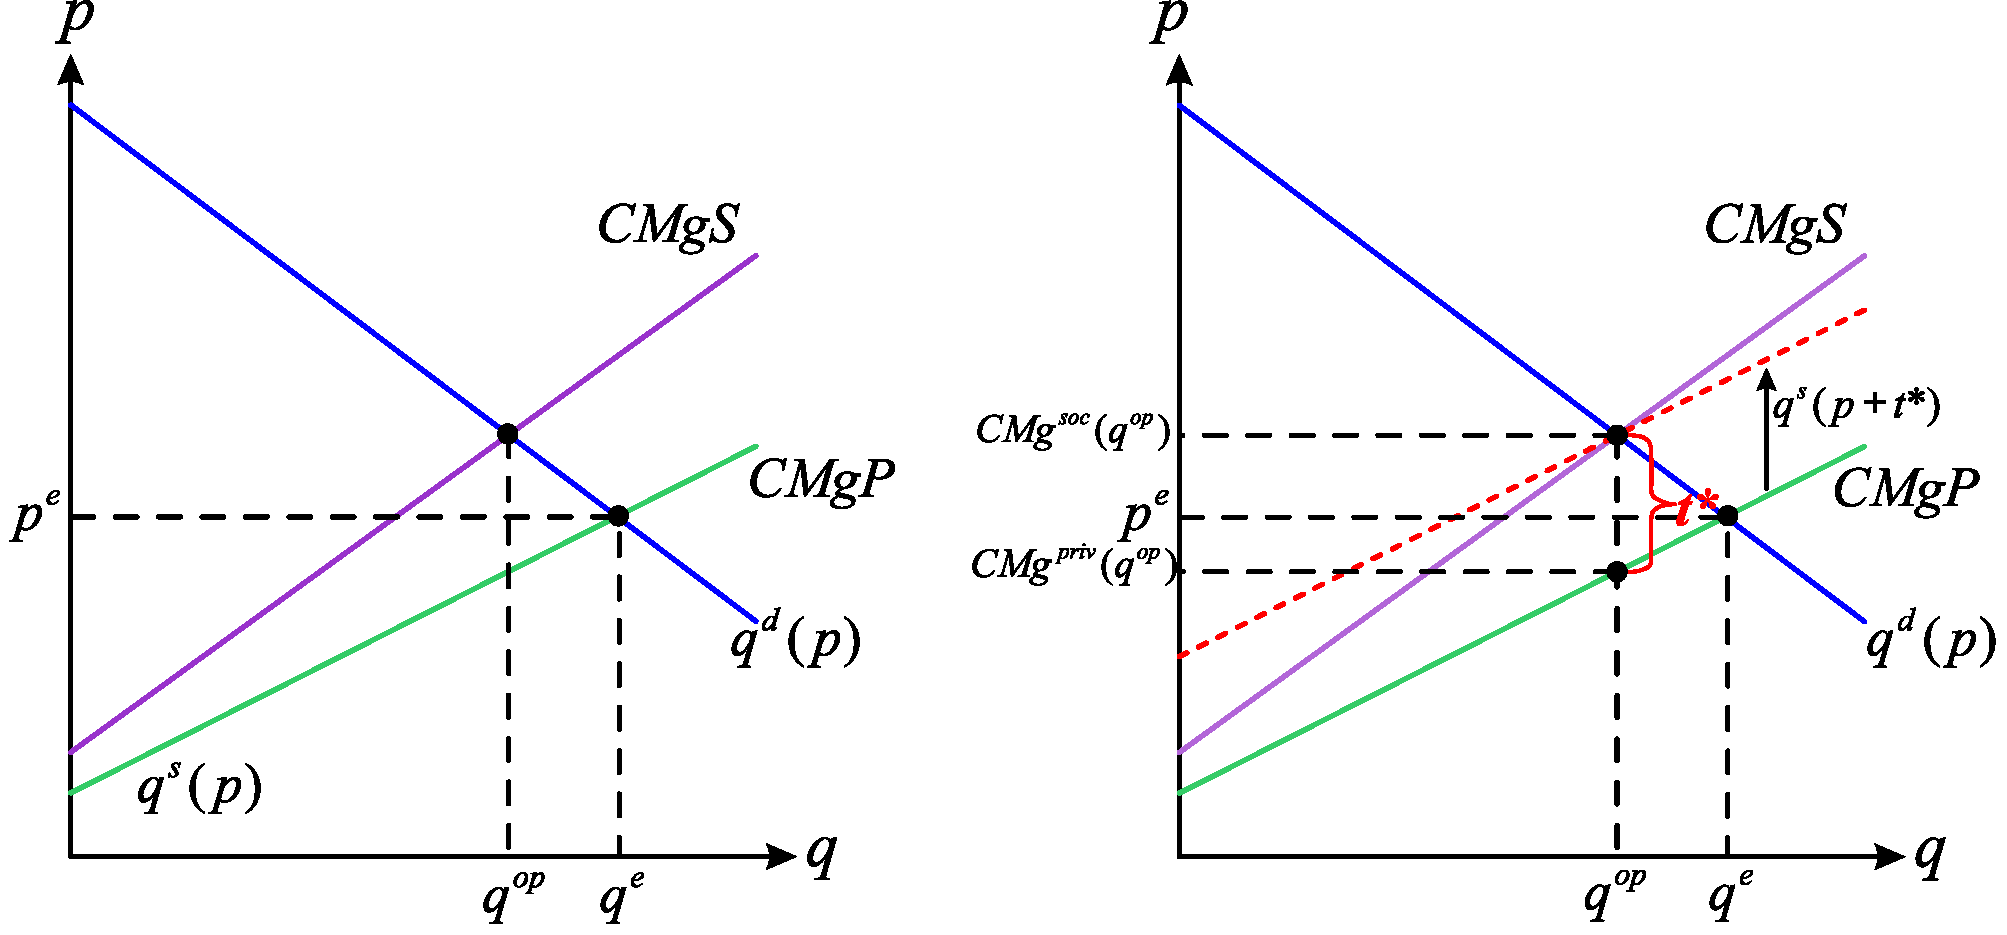
\includegraphics[width = 1\linewidth]{figures/impuestos.pdf}
	\end{center}
\end{frame}
%------------------------------------------------
\begin{frame}{Impuesto Pigouviano}
	\begin{itemize}
		\item El impuesto Pigouviano parece ser una solución simple
				\begin{itemize}
					\item El impuesto pagado = daño marginal
					\item El subsidio recibido = beneficio marginal
				\end{itemize}
		\item Pero hay limitaciones
				\begin{itemize}
					\item Los impuestos pueden necesitar ser diferenciados entre consumidores, empresas y bienes.
					\item Sin diferenciación suficiente, la externalidad sería corregida sólo parcialmente
					\item La intervención puede ser también requerida en los mercados de bienes relacionados
				\end{itemize}
		\item El impuesto debe ser visto como poner un precio a la externalidad.
	\end{itemize}
\end{frame}
%6) Eficiencia paretiana débil y fuerte ---------
	%====================================================================================
\section[Coase]{Teorema de Coase}
%====================================================================================

\begin{frame}{Teorema de Coase}
	\begin{itemize}
		\item El llamado ``Teorema de Coase'' propone que los agentes económicos resolverán los problemas de externalidad sin intervención.
		\item El Teorema puede formularse como:
			\emph{``En una econpmía competitiva, con información completa y costos de transacción nulos, la asignación de recursos será eficiente e invariable con respecto a las reglas legales de titularidad''}.
		\item Las reglas legales de titularidad (o \emph{derechos de propiedad}) determinan la propiedad en la economía.
		\item Coase ve las externalidades como surgidas por la ausencia de derechos de propiedad
			\begin{itemize}
				\item La contaminación ocurre cuando no hay derecho a aire limpio o agua limpia.
			\end{itemize}
		\item Si hubiera un derecho de propiedad, cualquiera que sufra una externalidad recibiría una compensación.
		\item La compensación es el precio por la externalidad.
		\item El intercambio competitivo asegura que surja el precio correcto y que se alcance la eficiencia.
	\end{itemize}
\end{frame}
%------------------------------------------------
\begin{frame}{Teorema de Coase}
	\begin{itemize}
		\item Coase ve las externalidades como surgidas por la ausencia de derechos de propiedad
			\begin{itemize}
				\item La contaminación ocurre cuando no hay derecho a aire limpio o agua limpia.
			\end{itemize}
		\item Si hubiera un derecho de propiedad, cualquiera que sufra una externalidad recibiría una compensación.
		\item La compensación es el precio por la externalidad.
		\item El intercambio competitivo asegura que surja el precio correcto y que se alcance la eficiencia.
		\item El Teorema también afirma que el equilibrio es invariable a la asignación de derechos de propiedad.
		\item Una empresa, ¿contaminará la atmósfera de una casa vecina?
			\begin{itemize}
				\item Sólo si el beneficio de hacerlo excede la compensación requerida por el propietario de la casa.
				\item Esto se aplica si la empresa tiene el derecho a contaminar o si el propietario de la casa tienenel derecho a aire limpio.
			\end{itemize}
	\end{itemize}
\end{frame}
%------------------------------------------------
\begin{frame}{Teorema de Coase}
	\begin{itemize}
		\item La distribución final de ingreso será diferente.
		\item El equilibrio no cambiará por la asignación de derechos de propiedad si no hay efectos ingreso.
		\item Las limitaciones prácticas del Teorema de Coase son:
			\begin{itemize}
				\item La carencia de derechos de propiedad claros.
				\item Los costos de transacción en alcanzar acuerdos de compensación
				\item Las implicancias de la negociación bilateral y la ineficiencia potencial con información incompleta.
				\item El poder de monopolio potencial.
			\end{itemize}
		\item El Teorema de Coase sugiere una resolución al problema de las externalidades pero hay razones por las cuales el mercado puede no funcionar.
	\end{itemize}
\end{frame}
%------------------------------------------------
\begin{frame}{Teorema de Coase}
	Volviendo al ejemplo:
		\begin{itemize}
			\item Supongamos que la piscigranja tenga derecho a tener agua pura, y lo vende para permitir que la suderurgia contamine.
			\item Sea $q$ el precio por unidad de contaminación.
		\end{itemize}
\end{frame}
%------------------------------------------------
\begin{frame}{Creación de mercados de derechos (Coase)}
	Los problemas de maximización serán:\\
		\begin{center}
			\begingroup
			\setlength{\tabcolsep}{10pt} % Default value: 6pt
			\renewcommand{\arraystretch}{1.5} % Default value: 1
				\begin{tabular}{ccc}
						\hline
					Para la acería & {} & Para la piscigranja\\
					$\M \limits_{s,x} \pi_s = p_ss - c_s(s,x) -qx$ & {} & $\M \limits_{f,x} \pi_f = p_f - c_f(f,x) +qx$\\
						\hline 
					\multicolumn{3}{c}{condiciones de primer orden} \\
					\hline
					$\frac{\partial \pi}{\partial s} = 0 \Leftrightarrow p_s - \frac{\partial c_s}{\partial s} = 0$ & {} & $\frac{\partial \pi}{\partial f} = 0 \Leftrightarrow p_f - \frac{\partial c_f}{\partial f} = 0$\\
					$p_s = \frac{\partial c_s}{\partial s}$ & {} & $p_f = \frac{\partial c_f}{\partial f}$\\
					$\frac{\partial \pi}{\partial x} = 0 \Leftrightarrow - \frac{\partial c_s}{\partial x} - q = 0$ &{} & 	$\frac{\partial \pi}{\partial x} = 0 \Leftrightarrow - \frac{\partial c_f}{\partial x} + q = 0$\\
					$q = -\frac{\partial c_s}{\partial x}$& {} & $q = \frac{\partial c_f}{\partial x}$ \\
						\hline
				\end{tabular}
			\endgroup
		\end{center}
	En consecuencia, se llega a las condiciones de eficiencia:
		$$-\frac{\partial c_s}{\partial x}=\frac{\partial c_f}{\partial x}$$
\end{frame}
%------------------------------------------------
\begin{frame}{Equilibrio general competitivo y externalidad negativa}
	\begin{center}
		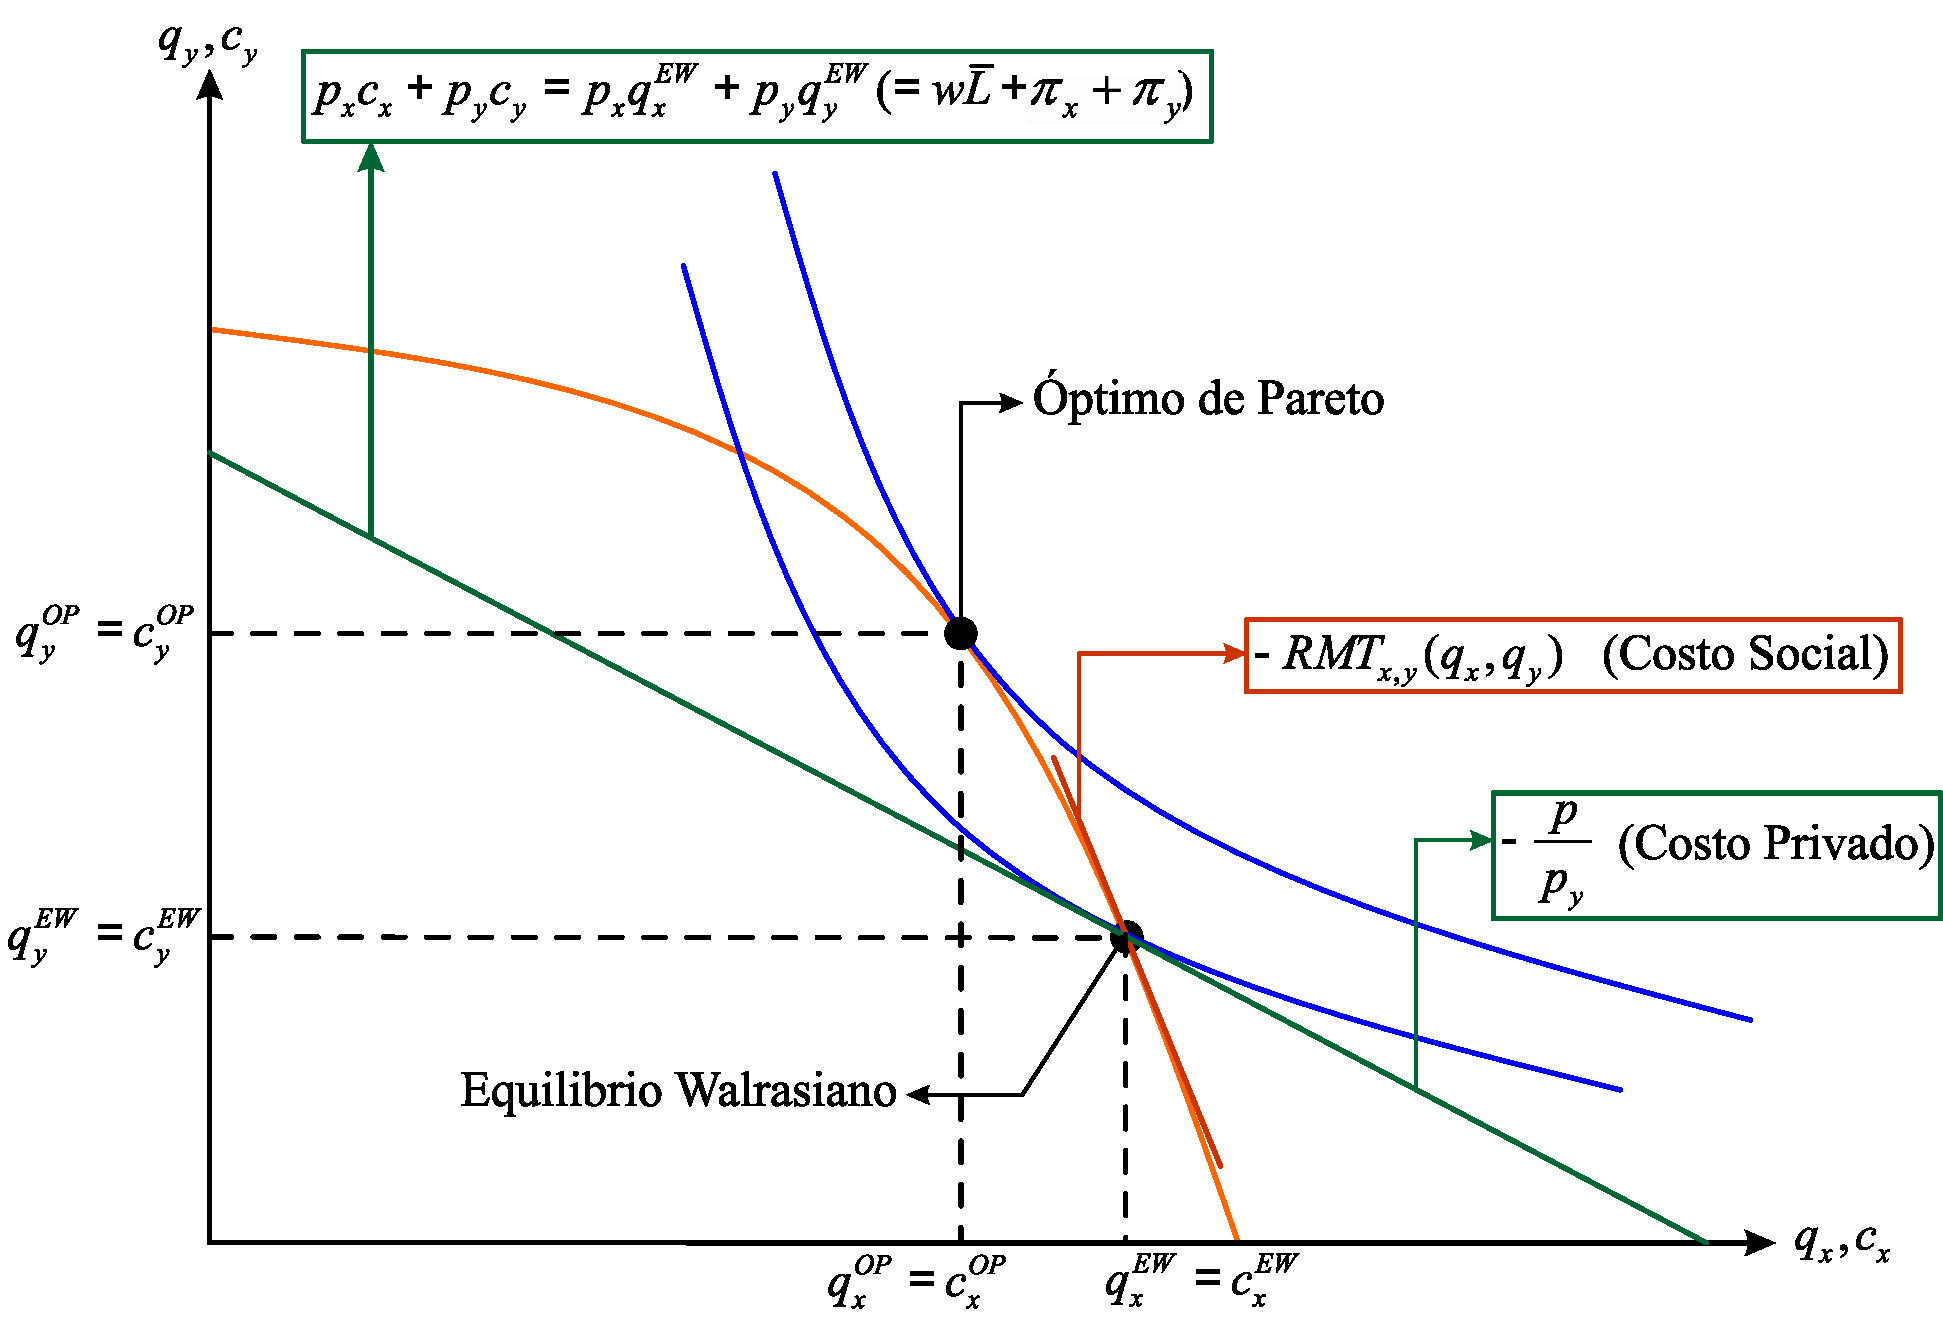
\includegraphics[width = 1\linewidth]{figures/equilibrio.pdf}
	\end{center}
\end{frame}

%------------------------------------------------------------------------------------
\subsection{Más sobre el Teorema de Coase}
%------------------------------------------------------------------------------------
\begin{frame}{Más sobre el Teorema de Coase}
Ejemplo del panadero y del médico:
	\begin{itemize}
		\item La máquina del panadero produce ruido y vibraciones que molestan a un médico vecino.
		\item Evitar el daño al médico implica infligir daño al panadero.
		\item Problema de fondo: ¿vale la pena reducir la producción de dulces para aumentar la de servicios médicos?
		\item El médico demandó al panadero y la corte le dio la razón.
		\item Pero para Coase, el médico habría aceptado que siga funcionando la máquina del panadero, si el panadero hubiere pagado una suma mayor a la pérdida del médico.
	\end{itemize}	
\end{frame}
%------------------------------------------------
\begin{frame}{Más sobre el Teorema de Coase}
Ejemplo del panadero y del médico:
	\begin{itemize}
		\item Igual, el panadero habría aceptado pagar un monto menor a su pérdida por el cambio o reducción de su nivel de producción.
		\item Según Coase, la solución sólo dependía de si el uso continuo de la maquinaria añade al ingreso del panadero más de lo que resta al ingreso del doctor.
		\item Si ambos hubiesen llegado a un acuerdo sin mayor costo, la decisión de cuál mantenía su actividad dependía de los ingresos involucrados.
		\item En consecuencia, la decisión del juez era irrelevante.
	\end{itemize}
\end{frame}
%------------------------------------------------
\begin{frame}{Gráficamente}
	\begin{multicols}{2}
		\begin{itemize}
			\item $BMNP$= Beneficio Marginal Neto Privado = beneficio adicional que obtiene la panadería por unidad producida.
			\item $DM$ = Daño Marginal = perjuicio adicional que la panadería provoca al médico.
		\end{itemize}
		
		\begin{center}
			\begin{tikzpicture}[scale=1]
	% Formación de la caja
		% Consumidor A
			\draw[->] (0.5,0.5) node[align=center, below left] {\footnotesize $O_A$} -- (0.5,4.5) node[align=center, above] {\footnotesize $x_{2}^{A}$};
			\draw[->] (0.5,0.5) -- (8.5,0.5) node[align=center, right] {\footnotesize $x_{1}^{A}$};
	
		%Consumidor B
			\draw[->] (8,4) node[align=center, above right] {\footnotesize $O_B$} -- (0,4) node[align=center, left] {\footnotesize $x_{2}^{B}$};
			\draw[->] (8,4) -- (8,0) node[align=center, below] {\footnotesize $x_{2}^{B}$};
	
	% Intersección de una dotación
		\draw[dashed] (6,4) node[above] {\footnotesize $x_{1}^{B}$} -- (6,0.5) node[below] {\footnotesize $x_{1}^{A}$};
		\draw[dashed] (0.5,2) node[left] {\footnotesize $x_{2}^{A}$} -- (8,2)node[right] {\footnotesize $x_{2}^{B}$};
	
	% Llaves
		\draw [decorate,decoration={brace,amplitude=5pt},xshift=-4pt,yshift=0pt] (6.1,-0.05) -- (0.7,-0.05);
		\node [right] at (3,-0.4) {$w_{1}^{A}$};
	
		\draw [decorate,decoration={brace,amplitude=5pt},xshift=-4pt,yshift=0pt] (6.2,4.6) --(8.2,4.6);
		\node [right] at (6.78,5.1) {$w_{1}^{B}$};
		
		\draw [decorate,decoration={brace,amplitude=5pt},xshift=-4pt,yshift=0pt] (-0.05,0.5) --(-0.05,2);
		\node [left] at (-0.3,1.27) {$w_{2}^{A}$};
		
		\draw [decorate,decoration={brace,amplitude=5pt},xshift=-4pt,yshift=0pt] (8.8,4) --(8.8,2);
		\node [right] at (8.8,3.05) {$w_{2}^{B}$};
		
		\draw [decorate,decoration={brace,amplitude=5pt},xshift=-4pt,yshift=0pt] (8,-0.6) -- (0.7,-0.6);
		\node [right] at (2.3,-1.05) {$x_{1}^{A}+x_{1}^{B}=\overline{w}_1=w_{1}^{A}+w_{1}^{B}$};
		
		\draw [decorate,decoration={brace,amplitude=5pt},xshift=-4pt,yshift=0pt] (-0.8,0.5) --(-0.8,4);
		\node [left,rotate=90] at (-1.4,4.4) {$x_{2}^{A}+x_{2}^{B}=\overline{w}_2=w_{2}^{A}+w_{2}^{B}$};
\end{tikzpicture}
		\end{center}
	\end{multicols}
\end{frame}
%------------------------------------------------
\begin{frame}{Si el panadero no fuese declarado responsable:}
	\begin{multicols}{2}
		\begin{itemize}
			\item $Q\ast$ = nivel de producción que maximiza el beneficio del panadero.
			\item Si disminuye $Q$:
				\begin{itemize}
					\item Hay una pequeña disminución del beneficio del panadero.
					\item Hay un mayor beneficio para el médico
				\end{itemize}
			\item Por tanto, el médico tiene incentivos para compensar al panadero por la menor producción.
		\end{itemize}
		
		\begin{center}
			\begin{tikzpicture}
	% FPP
		% Ejes
			\draw[->] (10,0)-- (10,5) node[align=center, above] {\footnotesize $q_{y}$};
			\draw[->] (10,0) -- (15,0) node[align=center, right] {\footnotesize $q_{x}$};
		% Curva
			\draw [orange] (10,4.5) ..controls (13,3.5) and (14,2.5) .. (14.5,0);
			
	% Minicaja
		% Intersección
			\draw [<->] (9.5,2.7) -- (13.29,2.7) node [below right, scale=0.7] {$O_B$} -- (13.29,-0.5);
			\draw [<->] (10,3.2) -- (10,0) node [left, scale=0.7] {$O_A$} -- (13.79,0);
		% Puntos
			\draw[black, fill=black] (13.29,2.7) circle[radius=0.05] node [above right, scale=0.7] {$\overline{Q}_G$};
		% Curva de contrato
			\draw [purple] (10,0) ..controls (11.29,0.2) and (12.29,2.4) .. (13.29,2.7);
			\draw [blue] (10.2,2.3) ..  controls (11.7,1.4) and (11.9,1.15) .. (12.1,0.08);
			\draw [red] (11.2,2.6) ..  controls (11.2,1.6) and (11.8,0.7) .. (13.2,0.2);
		% Pendientes
			\draw (11.27,4.99) -- (14.68,1.13);
			\draw (10.36,2.7) -- (12.74,0);
		% Símbolo de paraleleas
			\draw (10.55,2.35) -- (10.69,2.48);
			\draw (10.59,2.3) -- (10.74,2.43);
			
			\draw (12.19,3.8) -- (12.34,3.93);
			\draw (12.24,3.75) -- (12.38,3.88);
		% 	Etqiueta
			\draw (15, 3.5) node {$RMS_A = RMS_B = RMT$};
		% Punto
			\draw[black, fill=black] (11.67,1.22) circle[radius=0.05] node [right, scale=0.7] {$\overline{G}$};
\end{tikzpicture}
		\end{center}
	\end{multicols}
\end{frame}
%------------------------------------------------
\begin{frame}{Si el panadero no fuese declarado responsable:}
	\begin{multicols}{2}
		\begin{itemize}
			\item $A$ = ganancia del médico, luego de compensar al panadero.
			\item $B$ = pérdida del panadero que será compensada por el médico
		\end{itemize}
		
		\begin{center}
			\begin{tikzpicture}
	% FPP
		% Ejes
			\draw[->] (10,0)-- (10,5) node[align=center, above] {\footnotesize $q_{y}$};
			\draw[->] (10,0) -- (15,0) node[align=center, right] {\footnotesize $q_{x}$};
		% Curva
			\draw [orange] (10,4.5) ..controls (13,3.5) and (14,2.5) .. (14.5,0);
			
	% Minicaja
		% Intersección
			\draw [<->] (9.5,2.7) -- (13.29,2.7) node [below right, scale=0.7] {$O_B$} -- (13.29,-0.5);
			\draw [<->] (10,3.2) -- (10,0) node [left, scale=0.7] {$O_A$} -- (13.79,0);
		% Puntos
			\draw[black, fill=black] (13.29,2.7) circle[radius=0.05] node [above right, scale=0.7] {$\overline{Q}_G$};
		% Curva de contrato
			\draw [purple] (10,0) ..controls (11.29,0.2) and (12.29,2.4) .. (13.29,2.7);
			\draw [blue] (10.2,2.3) ..  controls (11.7,1.4) and (11.9,1.15) .. (12.1,0.08);
			\draw [red] (11.2,2.6) ..  controls (11.2,1.6) and (11.8,0.7) .. (13.2,0.2);
		% Pendientes
			\draw (11.27,4.99) -- (14.68,1.13);
			\draw (10.36,2.7) -- (12.74,0);
		% Símbolo de paraleleas
			\draw (10.55,2.35) -- (10.69,2.48);
			\draw (10.59,2.3) -- (10.74,2.43);
			
			\draw (12.19,3.8) -- (12.34,3.93);
			\draw (12.24,3.75) -- (12.38,3.88);
		% 	Etqiueta
			\draw (15, 3.5) node {$RMS_A = RMS_B = RMT$};
		% Punto
			\draw[black, fill=black] (11.67,1.22) circle[radius=0.05] node [right, scale=0.7] {$\overline{G}$};
\end{tikzpicture}
		\end{center}
	\end{multicols}
\end{frame}
%------------------------------------------------
\begin{frame}{Si el panadero no fuese declarado responsable:}
	\begin{multicols}{2}
		\begin{itemize}
			\item Mientras $A >B$, el médico tiene incentivos para compensar, llegándose al óptimo.
			\item Más allá de $Q^S$, al médico no le conviene compensar
		\end{itemize}
		
		\begin{center}
			\begin{tikzpicture}[scale=1.1]
	% Formación de la caja
		% Consumidor A
			\draw[->] (0.5,0.5) node[align=center, below left] {\footnotesize $O_J$} -- (0.5,4.5) node[align=center, above] {\footnotesize $6R$};
			\draw[->] (0.5,0.5) -- (8.5,0.5) node[align=center, right] {\footnotesize $10A$};
		
		% Consumidor B
			\draw[->] (8,4) node[align=center, above right] {\footnotesize $O_K$} -- (0,4) node[align=center, left] {\footnotesize $10A$};
			\draw[->] (8,4) -- (8,0) node[align=center, below] {\footnotesize $6R$};
			
		% Flechas
			\node[draw, single arrow,
				minimum height=22mm, minimum width=1mm,
				single arrow head extend=1.5mm,
				anchor=west, red, scale=0.5, rotate=-90,transform shape] at (8.4,2.87) {\small Ropa de Karen};
				
			\node[draw, single arrow,
				minimum height=22mm, minimum width=1mm,
				single arrow head extend=1.5mm,
				anchor=west, blue, scale=0.5, rotate=90,transform shape] at (0.1,1.57) {\small Ropa de Jaime};
				
			\node[draw, single arrow,
				minimum height=22mm, minimum width=1mm,
				single arrow head extend=1.5mm,
				anchor=west, red, scale=0.5, rotate=180,transform shape] at (5,4.3) {\rotatebox {180} {\small Alimento de Karen}};
			
			\node[draw, single arrow,
				minimum height=22mm, minimum width=1mm,
				single arrow head extend=1.5mm,
				anchor=west, blue, scale=0.5,transform shape] at (3.5,0.2) {\small Alimento de Jaime};
		
	% Curvas de indiferencia
		\begin{axis}[
					hide axis,
					xmin=0, xmax=10, 
					ymin=0, ymax=10,
					ytick=\empty,
					]
			
			% Área sombreada
				\fill [pattern=crosshatch dots,pattern color=green!60!white] (axis cs:4.07,6.462) to [bend right=34] coordinate[pos=0.5] (l_i) (axis cs:8.43,1.57) to (axis cs:8.42,1.56) to [bend right=34] coordinate[pos=0] (l_i) (axis cs:4,6.461);;
			
			% Curvas de indiferencia
				% Agente A
					\draw [blue] (axis cs:4,6.9) to [bend right=40] coordinate[pos=1] (l_i) (axis cs:9,1.5);
					\draw [blue] (axis cs:4.8,6.9) to [bend right=40] coordinate[pos=1] (l_i) (axis cs:9,2.3);
					\draw [blue] (axis cs:6.2,6.9) to [bend right=40] coordinate[pos=1] (l_i) (axis cs:9,3.7);
				
				% Agente B
					\draw [red] (axis cs:8.5,1) to [bend right=40] coordinate[pos=0.5] (l_i) (axis cs:3.6,6.5);
					\draw [red] (axis cs:8,1) to [bend right=40] coordinate[pos=0.5] (l_i) (axis cs:3.6,6);
					\draw [red] (axis cs:7.1,1) to [bend right=40] coordinate[pos=0.5] (l_i) (axis cs:3.6,5.1);
					\draw [red] (axis cs:6.3,1) to [bend right=40] coordinate[pos=0.5] (l_i) (axis cs:3.6,4.3);
		\end{axis}
	
	% Punto
		\draw[black, fill=black] (5.775,0.89) circle[radius=0.05] node [above right] {$C$};
		\draw[black, fill=black] (5.26,1.47) circle[radius=0.05] node [above right] {$D$};
		\draw[black, fill=black] (4.1,2.2) circle[radius=0.05] node [above right] {$E$};
		\draw[black, fill=black] (3.7,1.9) circle[radius=0.05] node [below left] {$F$};
		\draw[black, fill=black] (4.82,2.7) circle[radius=0.05] node [above right] {$G$};
	
	% Etiqueta de función de utilidad
		% Agente A
			\node [blue, scale=0.18mm]  at (6.35,0.8) {$u_{J}^{1}$};
			\node [blue, scale=0.18mm]  at (6.35,1.27) {$u_{J}^{1}$};
			\node [blue, scale=0.18mm]  at (6.35,2.06) {$u_{J}^{1}$};
			
		% Agente B
			\node [red, scale=0.18mm]  at (2.3,3.8) {$u_{K}^{1}$};
			\node [red, scale=0.18mm]  at (2.3,3.5) {$u_{K}^{2}$};
			\node [red, scale=0.18mm]  at (2.3,3) {$u_{K}^{3}$};
			\node [red, scale=0.18mm]  at (2.3,2.55) {$u_{K}^{4}$};
	
\end{tikzpicture}
		\end{center}
	\end{multicols}
\end{frame}
%------------------------------------------------
\begin{frame}{Si el panadero fuese declarado responsable:}
	\begin{multicols}{2}
		\begin{itemize}
			\item El médico maximiza beneficios en Q*.
			\item Si el médico recibe un poco de ruido
				\begin{itemize}
					\item Hay un pequeño perjuicio para él.
					\item Pero un gran beneficio para el panadero
				\end{itemize}
			\item Por tanto, el panadero tiene incentivos para compensar al médico, para poder producir.
		\end{itemize}
		
		\begin{center}
			\begin{tikzpicture}[scale=1.1]
	% Formación de la caja
		% Consumidor A
			\draw[->] (0.5,0.5) node[align=center, below left] {\footnotesize $O_J$} -- (0.5,4.5) node[align=center, above] {\footnotesize $6R$};
			\draw[->] (0.5,0.5) -- (8.5,0.5) node[align=center, right] {\footnotesize $10A$};
		
		%Consumidor B
			\draw[->] (8,4) node[align=center, above right] {\footnotesize $O_K$} -- (0,4) node[align=center, left] {\footnotesize $10A$};
			\draw[->] (8,4) -- (8,0) node[align=center, below] {\footnotesize $6R$};
		
		% Flechas
			\node[draw, single arrow,
					minimum height=22mm, minimum width=1mm,
					single arrow head extend=1.5mm,
					anchor=west, red, scale=0.5, rotate=-90,transform shape] at (8.4,2.87) {\small Ropa de Karen};
			
			\node[draw, single arrow,
					minimum height=22mm, minimum width=1mm,
					single arrow head extend=1.5mm,
					anchor=west, blue, scale=0.5, rotate=90,transform shape] at (0.1,1.57) {\small Ropa de Jaime};
			
			\node[draw, single arrow,
					minimum height=22mm, minimum width=1mm,
					single arrow head extend=1.5mm,
					anchor=west, red, scale=0.5, rotate=180,transform shape] at (5,4.3) {\rotatebox {180} {\small Alimento de Karen}};
			
			\node[draw, single arrow,
					minimum height=22mm, minimum width=1mm,
					single arrow head extend=1.5mm,
					anchor=west, blue, scale=0.5,transform shape] at (3.5,0.2) {\small Alimento de Jaime};
		
	% Curvas de indiferencia
		\begin{axis}[
					hide axis,
					xmin=0, xmax=10, 
					ymin=0, ymax=10,
					ytick=\empty,
					]
			
			% Curvas de indiferencia
				% Agente A
					\draw [blue] (axis cs:4,6.9) to [bend right=40] coordinate[pos=1] (l_i) (axis cs:9,1.5);
					\draw [blue] (axis cs:4.8,6.9) to [bend right=40] coordinate[pos=1] (l_i) (axis cs:9,2.3);
					\draw [blue] (axis cs:6.2,6.9) to [bend right=40] coordinate[pos=1] (l_i) (axis cs:9,3.7);
				
				% Agente B
					\draw [red] (axis cs:8.5,1) to [bend right=40] coordinate[pos=0.5] (l_i) (axis cs:3.6,6.5);
					\draw [red] (axis cs:7.1,1) to [bend right=40] coordinate[pos=0.5] (l_i) (axis cs:3.6,5.1);
					\draw [red] (axis cs:6.3,1) to [bend right=40] coordinate[pos=0.5] (l_i) (axis cs:3.6,4.3);
		\end{axis}

	
	% Curva de contrato
		\draw  [purple, very thick] (0.5,0.5) ..controls (1.8,1.5) and (2.5,0.7) .. (3.7,1.9) .. controls (3.8,2.1) .. (4.1,2.2) .. controls (4.5,2.3) .. (4.82,2.7) ..controls (6.12,3.7) and (6.8,2.8) .. (8,4);
	
	% Punto
		\draw[black, fill=black] (4.1,2.2) circle[radius=0.05] node [above] {$E$};
		\draw[black, fill=black] (3.7,1.9) circle[radius=0.05] node [below] {$F$};
		\draw[black, fill=black] (4.82,2.7) circle[radius=0.05] node [above] {$G$};
	
	% Etiqueta de función de utilidad
		% Agente A
			\node [blue, scale=0.18mm]  at (6.35,0.8) {$u_{J}^{1}$};
			\node [blue, scale=0.18mm]  at (6.35,1.27) {$u_{J}^{1}$};
			\node [blue, scale=0.18mm]  at (6.35,2.06) {$u_{J}^{1}$};
		
		% Agente B
			\node [red, scale=0.18mm]  at (2.3,3.8) {$u_{K}^{1}$};
			\node [red, scale=0.18mm]  at (2.3,3.5) {$u_{K}^{2}$};
			\node [red, scale=0.18mm]  at (2.3,3) {$u_{K}^{3}$};
			\node [red, scale=0.18mm]  at (2.3,2.55) {$u_{K}^{4}$};
			
	% Flechas
		\node[draw, single arrow,
				minimum height=22mm, minimum width=1mm,
				single arrow head extend=1.5mm,
				anchor=west, purple, scale=0.5,,transform shape] at (0.8,1.4) {Curva de contrato};
\end{tikzpicture}
		\end{center}
	\end{multicols}
\end{frame}
%------------------------------------------------
\begin{frame}{Si el panadero fuese declarado responsable:}
	\begin{multicols}{2}
		\begin{itemize}
			\item $A$ = ganancia del panadero, luego de compensar al médico.
			\item $B$ = pérdida del médico  que será compensada por el panadero.
			\item Mientras $A >B$, el panadero tiene incentivos para compensar, llegándose al óptimo.
			\item Más allá de $Q^s$, al panadero no le conviene  compensar.
		\end{itemize}
		
		\begin{center}
			\begin{tikzpicture}[scale=1.1]
	% Formación de la caja
		% Consumidor A
			\draw[->] (0.5,0.5) node[align=center, below left] {\footnotesize $O_J$} -- (0.5,4.5) node[align=center, above] {\footnotesize $6R$};
			\draw[->] (0.5,0.5) -- (8.5,0.5) node[align=center, right] {\footnotesize $10A$};
		
		%Consumidor B
			\draw[->] (8,4) node[align=center, above right] {\footnotesize $O_K$} -- (0,4) node[align=center, left] {\footnotesize $10A$};
			\draw[->] (8,4) -- (8,0) node[align=center, below] {\footnotesize $6R$};
		
		% Flechas
			\node[draw, single arrow,
					minimum height=22mm, minimum width=1mm,
					single arrow head extend=1.5mm,
					anchor=west, red, scale=0.5, rotate=-90,transform shape] at (8.4,2.87) {\small Ropa de Karen};
			
			\node[draw, single arrow,
					minimum height=22mm, minimum width=1mm,
					single arrow head extend=1.5mm,
					anchor=west, blue, scale=0.5, rotate=90,transform shape] at (0.1,1.57) {\small Ropa de Jaime};
			
			\node[draw, single arrow,
					minimum height=22mm, minimum width=1mm,
					single arrow head extend=1.5mm,
					anchor=west, red, scale=0.5, rotate=180,transform shape] at (5,4.3) {\rotatebox {180} {\small Alimento de Karen}};
			
			\node[draw, single arrow,
					minimum height=22mm, minimum width=1mm,
					single arrow head extend=1.5mm,
					anchor=west, blue, scale=0.5,transform shape] at (3.5,0.2) {\small Alimento de Jaime};
		
	% Curvas de indiferencia
		\begin{axis}[
					hide axis,
					xmin=0, xmax=10, 
					ymin=0, ymax=10,
					ytick=\empty,
					]
			
			% Curvas de indiferencia
				% Agente A
					\draw [blue] (axis cs:4,6.9) to [bend right=40] coordinate[pos=1] (l_i) (axis cs:9,1.5);
					\draw [blue] (axis cs:4.8,6.9) to [bend right=40] coordinate[pos=1] (l_i) (axis cs:9,2.3);
					\draw [blue] (axis cs:6.2,6.9) to [bend right=40] coordinate[pos=1] (l_i) (axis cs:9,3.7);
				
				% Agente B
					\draw [red] (axis cs:8.5,1) to [bend right=40] coordinate[pos=0.5] (l_i) (axis cs:3.6,6.5);
					\draw [red] (axis cs:7.1,1) to [bend right=40] coordinate[pos=0.5] (l_i) (axis cs:3.6,5.1);
					\draw [red] (axis cs:6.3,1) to [bend right=40] coordinate[pos=0.5] (l_i) (axis cs:3.6,4.3);
		\end{axis}

	
	% Curva de contrato
		\draw  [purple, very thick] (0.5,0.5) ..controls (1.8,1.5) and (2.5,0.7) .. (3.7,1.9) .. controls (3.8,2.1) .. (4.1,2.2) .. controls (4.5,2.3) .. (4.82,2.7) ..controls (6.12,3.7) and (6.8,2.8) .. (8,4);
	
	% Punto
		\draw[black, fill=black] (4.1,2.2) circle[radius=0.05] node [above] {$E$};
		\draw[black, fill=black] (3.7,1.9) circle[radius=0.05] node [below] {$F$};
		\draw[black, fill=black] (4.82,2.7) circle[radius=0.05] node [above] {$G$};
	
	% Etiqueta de función de utilidad
		% Agente A
			\node [blue, scale=0.18mm]  at (6.35,0.8) {$u_{J}^{1}$};
			\node [blue, scale=0.18mm]  at (6.35,1.27) {$u_{J}^{1}$};
			\node [blue, scale=0.18mm]  at (6.35,2.06) {$u_{J}^{1}$};
		
		% Agente B
			\node [red, scale=0.18mm]  at (2.3,3.8) {$u_{K}^{1}$};
			\node [red, scale=0.18mm]  at (2.3,3.5) {$u_{K}^{2}$};
			\node [red, scale=0.18mm]  at (2.3,3) {$u_{K}^{3}$};
			\node [red, scale=0.18mm]  at (2.3,2.55) {$u_{K}^{4}$};
			
	% Flechas
		\node[draw, single arrow,
				minimum height=22mm, minimum width=1mm,
				single arrow head extend=1.5mm,
				anchor=west, purple, scale=0.5,,transform shape] at (0.8,1.4) {Curva de contrato};
\end{tikzpicture}
		\end{center}
	\end{multicols}
\end{frame}
%------------------------------------------------
\begin{frame}{¿En qué casos si son relevantes las decisiones del Estado?}
	\begin{itemize}
		\item Cuando los costos de transacción son altos.
		\item Ejemplo: Aviones que hacen ruido en una zona residencial cercana al aeropuerto.
		\item En esos casos, la asignación de derechos que decida el Estado, debe basarse en un análisis económico para decidir la solución menos costosa.
	\end{itemize}
\end{frame}
%7) Ley de Walras -------------------------------
	%====================================================================================
\section[Walras]{Ley de Walras}
%====================================================================================

\begin{frame}{Intercambio de mercado: Walras}
	Walras analizó el intercambio de bienes por medio de mercados en los que para todos los bienes está definido un precio al cual todos los agentes pueden comprar o vender el bien. \\
		\medskip
	Se analiza un proceso de intercambio cóncreto: reproduce el resultado de un mecanismo competitivo. \\
		\medskip
	\textbf{Descentralización mediante precios.}
		\begin{itemize}
			\item Para poder hablar de solución \textbf{``competitiva''} hay que suponer que los agentes conocen a que precios se intercambian los bienes.
				\begin{itemize}
					\item Existe una tercera persona \textbf{``el subastados walrasiano''}, que elige los precios y los anuncia a los agentes y estos, a su vez, anuncian que cantidades desean comprar y/o vender.
				\end{itemize}
		\end{itemize}
\end{frame}
%------------------------------------------------
\begin{frame}{Los precios y las restricciones presupuestales}
	\textbf{Supuesto}: cada consumidor toma los precios como dados y determina su demanda de forma que maximice su bienestar sujeto a que, a esos mismos precios.\\
		\medskip
	En otras palabras, los agentes son precio-aceptantes, valoran lo que poseen a esos precios e intentan conseguir la mejor asignación asequible.\\
		\medskip
	\begin{table}[htb]
		\centering
			\begin{tabular}{m{0.3\linewidth}@{\quad $\leq$ \quad}m{0.3\linewidth}}
				Valor de consumo a precios de mercado & Valor de consumo a precios de mercado
			\end{tabular}
	\end{table}
		\medskip
	\textbf{¿Cómo se realiza el intercambio?}\\
	Con una determinada relación de precios, con la cual se valoriza las dotaciones iniciales de A y B; es decir:
		$$\overline{p} = \frac{p_1}{p_2}$$
\end{frame}
%------------------------------------------------
\begin{frame}{Los precios y las restricciones presupuestales}
		%\hspace{-0.5cm} \begin{tikzpicture}[transform canvas={scale=0.55}]
	% Formato de CAJA: Sola A
		\draw[->] (0.5,0.5) node[align=center, below left] {\footnotesize $O_A$} -- (0.5,4.8) node[align=center, above] {\footnotesize $x_{2}^{A}$};
		\draw[->] (0.5,0.5) -- (8.5,0.5) node[align=center, right] {\footnotesize $x_{1}^{A}$};
	
		% Rellenando el triangulo
			\fill [pattern=crosshatch dots,pattern color=orange!60!white] (0.5,4.3) -- (7.27,0.5) -- (0.5,0.5) -- (0.5,4.3) ;
			
		% Recta presupuestaria
			\draw (0.5,4.3) -- (7.27,0.5);
		
		% Punto
			\draw[black, fill=black] (4.6,2) circle[radius=0.1] node [ above right] {$w^{A}$};
		
		% Intersección de una dotación
			\draw[dashed] (4.6,2) -- (4.6,0.5) node[below] {\footnotesize $w_{1}^{A}$};
			\draw[dashed] (0.5,2) node[left] {\footnotesize $w_{2}^{A}$} -- (4.6,2);
		
		% Ecuación
			\node at (4.5, 3.7)  {$p_{1}x_{1}^{A}+p_{2}x_{2}^{A}=p_{1}w_{1}^{A}+p_{2}w_{2}^{A}$};
	
	% Formato de CAJA: Sola B
		\draw[->] (10.5,0.5) node[align=center, below left] {\footnotesize $O_B$} -- (10.5,4.8) node[align=center, above] {\footnotesize $x_{2}^{B}$};
		\draw[->] (10.5,0.5) -- (18.5,0.5) node[align=center, right] {\footnotesize $x_{1}^{B}$};
		
		% Rellenando el triangulo
			\fill [pattern=crosshatch dots,pattern color=green!50!white] (17.47,0.5) -- (10.5,4.41) -- (10.5,0.5) -- (17.47,0.5) ;
		
		% Recta presupuestaria
			\draw (17.47,0.5) -- (10.5,4.41);
		
		% Punto
			\draw[black, fill=black] (13.9,2.5) circle[radius=0.1] node [ above right] {$w^{B}$};
		
		% Intersección de una dotación
			\draw[dashed] (13.9,2.5) -- (13.9,0.5) node[below] {\footnotesize $w_{1}^{A}$};
			\draw[dashed] (10.5,2.5) node[left] {\footnotesize $w_{2}^{A}$} -- (13.9,2.5);
		
		% Ecuación
			\node at (14.5, 3.7)  {$p_{1}x_{1}^{B}+p_{2}x_{2}^{B}=p_{1}w_{1}^{B}+p_{2}w_{2}^{B}$};
	
	% Formato de CAJA: A y B conjunto
		\draw[->] (5.5,-5.5) node[align=center, below left] {\footnotesize $O_A$} -- (13.8,-5.5) node[align=center, right] {\footnotesize $x_{1}^{A}$};
		\draw[->] (5.5,-5.5) -- (5.5,-1.2) node[align=center, above] {\footnotesize $x_{2}^{A}$};
		
		\draw[->] (13,-2) node[align=center, above right] {\footnotesize $O_B$} -- (4.7,-2) node[align=center, left] {\footnotesize $x_{1}^{B}$};
		\draw[->] (13,-2) -- (13,-6.3) node[align=center, below] {\footnotesize $x_{2}^{B}$};
		
		% Rellenos
			% Naranaja
				\fill [pattern=crosshatch dots,pattern color=orange!60!white] (5.5,-1.7) -- (12.27,-5.5) -- (5.5,-5.5) -- (5.5,-1.7);
			
			% Verde
				\fill [pattern=crosshatch dots,pattern color=green!50!white] (6.04,-2) -- (13,-2) -- (13,-5.91) -- (6.04,-2) ;
		
		% Intersectando
			% Vertical
				\draw[dashed] (9.6, -2)  node[above] {\footnotesize $w_{1}^{B}$} -- (9.6,-5.5) node[below] {\footnotesize $w_{1}^{A}$};
			
			% Horizontal
				\draw[dashed] (5.5,-4) node[left] {\footnotesize $w_{2}^{A}$} -- (13,-4) node[right] {\footnotesize $w_{2}^{B}$};
		
		% punto
			\draw[black, fill=black, opacity=3] (9.6,-4) circle[radius=0.1] node [ above right] {$w$};
		
		% Recta presupuestaria
			\draw (5.5,-1.7) -- (13,-5.91);
\end{tikzpicture}
			Solo las canastas situadas en la recta presupuestaria son factibles para ambos consumidores simultaneamente, a los precios ``$P$''.\\
				\vspace{2.8cm}
			\begin{tikzpicture}[transform canvas={scale=0.55}]
	% Formato de CAJA: Sola A
		\draw[->] (0.5,0.5) node[align=center, below left] {\footnotesize $O_A$} -- (0.5,4.8) node[align=center, above] {\footnotesize $x_{2}^{A}$};
		\draw[->] (0.5,0.5) -- (8.5,0.5) node[align=center, right] {\footnotesize $x_{1}^{A}$};
	
		% Rellenando el triangulo
			\fill [pattern=crosshatch dots,pattern color=orange!60!white] (0.5,4.3) -- (7.27,0.5) -- (0.5,0.5) -- (0.5,4.3) ;
			
		% Recta presupuestaria
			\draw (0.5,4.3) -- (7.27,0.5);
		
		% Punto
			\draw[black, fill=black] (4.6,2) circle[radius=0.1] node [ above right] {$w^{A}$};
		
		% Intersección de una dotación
			\draw[dashed] (4.6,2) -- (4.6,0.5) node[below] {\footnotesize $w_{1}^{A}$};
			\draw[dashed] (0.5,2) node[left] {\footnotesize $w_{2}^{A}$} -- (4.6,2);
		
		% Ecuación
			\node at (4.5, 3.7)  {$p_{1}x_{1}^{A}+p_{2}x_{2}^{A}=p_{1}w_{1}^{A}+p_{2}w_{2}^{A}$};
	
	% Formato de CAJA: Sola B
		\draw[->] (10.5,0.5) node[align=center, below left] {\footnotesize $O_B$} -- (10.5,4.8) node[align=center, above] {\footnotesize $x_{2}^{B}$};
		\draw[->] (10.5,0.5) -- (18.5,0.5) node[align=center, right] {\footnotesize $x_{1}^{B}$};
		
		% Rellenando el triangulo
			\fill [pattern=crosshatch dots,pattern color=green!50!white] (17.47,0.5) -- (10.5,4.41) -- (10.5,0.5) -- (17.47,0.5) ;
		
		% Recta presupuestaria
			\draw (17.47,0.5) -- (10.5,4.41);
		
		% Punto
			\draw[black, fill=black] (13.9,2.5) circle[radius=0.1] node [ above right] {$w^{B}$};
		
		% Intersección de una dotación
			\draw[dashed] (13.9,2.5) -- (13.9,0.5) node[below] {\footnotesize $w_{1}^{A}$};
			\draw[dashed] (10.5,2.5) node[left] {\footnotesize $w_{2}^{A}$} -- (13.9,2.5);
		
		% Ecuación
			\node at (14.5, 3.7)  {$p_{1}x_{1}^{B}+p_{2}x_{2}^{B}=p_{1}w_{1}^{B}+p_{2}w_{2}^{B}$};
	
	% Formato de CAJA: A y B conjunto
		\draw[->] (5.5,-5.5) node[align=center, below left] {\footnotesize $O_A$} -- (13.8,-5.5) node[align=center, right] {\footnotesize $x_{1}^{A}$};
		\draw[->] (5.5,-5.5) -- (5.5,-1.2) node[align=center, above] {\footnotesize $x_{2}^{A}$};
		
		\draw[->] (13,-2) node[align=center, above right] {\footnotesize $O_B$} -- (4.7,-2) node[align=center, left] {\footnotesize $x_{1}^{B}$};
		\draw[->] (13,-2) -- (13,-6.3) node[align=center, below] {\footnotesize $x_{2}^{B}$};
		
		% Rellenos
			% Naranaja
				\fill [pattern=crosshatch dots,pattern color=orange!60!white] (5.5,-1.7) -- (12.27,-5.5) -- (5.5,-5.5) -- (5.5,-1.7);
			
			% Verde
				\fill [pattern=crosshatch dots,pattern color=green!50!white] (6.04,-2) -- (13,-2) -- (13,-5.91) -- (6.04,-2) ;
		
		% Intersectando
			% Vertical
				\draw[dashed] (9.6, -2)  node[above] {\footnotesize $w_{1}^{B}$} -- (9.6,-5.5) node[below] {\footnotesize $w_{1}^{A}$};
			
			% Horizontal
				\draw[dashed] (5.5,-4) node[left] {\footnotesize $w_{2}^{A}$} -- (13,-4) node[right] {\footnotesize $w_{2}^{B}$};
		
		% punto
			\draw[black, fill=black, opacity=3] (9.6,-4) circle[radius=0.1] node [ above right] {$w$};
		
		% Recta presupuestaria
			\draw (5.5,-1.7) -- (13,-5.91);
\end{tikzpicture}
				\vspace{4cm}
\end{frame}
%------------------------------------------------
\begin{frame}{Equilibrio General Walrasiano}
	Un equilibrio Walrasiano es una asignación $\left( x_{1}^{A},x_{2}^{A}, x_{1}^{B},x_{2}^{B}\right) $ , llamada asignación de equilibrio, y un vector de precios $\left( p_{1}, p_{2}\right) $ llamado vector de precios de equilibrio, tal que:
		\begin{itemize}
			\item Las economías domésticas eligen aquella cesta de consumo que maximizan su utilidad (demanda de bienes):
				$$\begin{array}{lll}
					RMS_{x_1,x_2}^{A}\left( x_{1}^{A},x_{2}^{A}\right)=\frac{p_{1}}{p_{2}} & {} & RMS_{x_1,x_2}^{B}\left( x_{1}^{B},x_{2}^{B}\right)=\frac{p_{1}}{p_{2}}\\ [0.5cm]
					p_{1}x_{1}^{A}+p_{2}x_{2}^{A}=p_{1}w_{1}^{A}+p_{2}w_{2}^{A} & {} & p_{1}x_{1}^{B}+p_{2}x_{2}^{B}=p_{1}w_{1}^{B}+p_{2}w_{2}^{B}
				\end{array}$$
			\item Los mercados de bienes están en equilibrio (demanda = oferta):
				$$\begin{array}{ccc}
					x_{1}^{A}+x_{1}^{B}=w_{1}^{A}+w_{1}^{B} & {} & x_{2}^{A}+x_{2}^{B}=w_{2}^{A}+w_{2}^{B}
				  \end{array}$$
		\end{itemize}
\end{frame}
%------------------------------------------------
\begin{frame}{Equilibrio General Walrasiano}
	La canasta $x^{A}$ maximiza el bienestar del agente $1$, sujeto a que el valor de su consumo no supere al de su dotación. Así mismo, la canastas $x^{B}$ hace lo mismo con el bienestar del agente 2.\\
		\begin{tikzpicture}[scale=1.1]
	% Formación de la caja
		% Consumidor A
			\draw[->] (0.5,0.5) node[align=center, below left] {\footnotesize $O_A$} -- (0.5,4.5) node[align=center, above] {\footnotesize $x_{2}^{A}$};
			\draw[->] (0.5,0.5) -- (8.5,0.5) node[align=center, right] {\footnotesize $x_{1}^{B}$};
		
		%Consumidor B
			\draw[->] (8,4) node[align=center, above right] {\footnotesize $O_B$} -- (0,4) node[align=center, left] {\footnotesize $x_{1}^{B}$};
			\draw[->] (8,4) -- (8,0) node[align=center, below] {\footnotesize $x_{2}^{B}$};
		
	% Intersección de una dotación
		% Demanda: X
			\draw[dashed] (5.2,4) node[above] {\footnotesize $x_{1}^{B}$} -- (5.2,0.5) node[below]{\footnotesize $x_{1}^{A}$};
			\draw[dashed] (0.5,2) node[left] {\footnotesize $x_{2}^{A}$} -- (8,2)node[right]{\footnotesize $x_{2}^{B}$};
		
		% Oferta: w
			\draw[dashed, opacity=0.4] (6,4) -- (6,0.5);
			\draw[dashed, opacity=0.4] (0.5,1.62)  -- (8,1.62);
			
				\draw (8,1.62)  node [right] {\footnotesize $w_{2}^{B}$};
				\draw (6,4)  node [above] {\footnotesize $w_{1}^{B}$};
				
				\draw (0.5,1.62)  node [left] {\footnotesize $w_{2}^{A}$};
				\draw (6,0.5)  node [below] {\footnotesize $w_{1}^{A}$};
	
	% Curvas de indiferencia
		\draw [blue] (3.5,4) .. controls (4.6,2) and (5.2,1.7) .. (8,1.4);
		\draw [red] (0.5,2.7) .. controls (4.915,2.515) and (5.915,2.015) .. (6.5,0.5);
	
	% Recta presupuestaria
		\draw (0.5,4.23) -- (8.36,0.5);
	
	% Puntos
		\draw[black, fill=black] (5.2,2) circle[radius=0.05] node [above right, scale=0.25mm] {$X$};
		\draw[black, fill=black] (6,1.62) circle[radius=0.05] node [above right, scale=0.25mm] {$W$};
		
	% Flecha y rectángulo
		\draw [->] (2.48,3.29) -- (2.67,3.69) node [left, scale = 0.3mm] {\footnotesize $p$};
		\draw [rotate around={-25:(2.48,3.29)}] (2.48,3.29) rectangle (2.6, 3.4);
\end{tikzpicture}
\end{frame}
%------------------------------------------------
\begin{frame}{Equilibrio General Walrasiano}
	Cada agente (considerando los precios como dados) se encuentra feliz con el resultado del intercambio (porque a esos precios y con su dotación inicial, cada agente no puede estar mejor), y además el intercambio puede realizarse (nadie está tratando de comprar o vender sin poder hacerlo)
\end{frame}
%------------------------------------------------
\begin{frame}{Equilibrio General Walrasiano}
	Como coinciden la pendientes de la recta presupuestal con las RMS, se tiene
		$$RMS_{x_1,x_2}^{A}\left( x_{1}^{A},x_{2}^{A}\right)  =  RMS_{x_1,x_2}^{B}\left( x_{1}^{B},x_{2}^{B}\right)  =  \frac{p_{1}}{p_{2}}$$
	Esto representa la condición de consumo eficiente (respuesta al problema de cómo asignar eficientemente los bienes entre los consumidores).
\end{frame}
%------------------------------------------------
\begin{frame}{Ley de Walras}
	Se define la función de exceso de demanda del bien $k$ para el consumidor $i$ como
		$$e_{ik}(p)=x_{ik}(p)-\overline{w}_{ik}$$
	Entonces
		$$e_{11}(p) + e_{21}(p)=0$$
		$$e_{12}(p) + e_{22}(p)=0$$
	Finalmente definimos la función de exceso de demanda agregada del bien $k$:
		$$z_{k}(p) = e_{1k}(p)+e_{2k}(p)$$
\end{frame}
%------------------------------------------------
\begin{frame}{Ley de Walras}
	El equilibrio walrasiano se puede definir entonces como un vector de precios $p^*$ y una asignación $x^*$, tal que
		$$z_{k}(p^*)=0, k=1,2$$
	Entonces, la Ley de Walras dice que la suma del valor de las funciones de exceso de demanda agregada es idénticamente igual a cero:
		$$\forall p, p_1z_1(p)+p_2z_2(p)=0$$
\end{frame}
%------------------------------------------------
\begin{frame}{Ley de Walras: Demostración}
		$$\forall p, p_1x_{11}(p)+p_2z_{12}(p)=p_1w_{11}+p_2w_{12}$$
	Para el consumidor 1, cualquier canasta de consumo, dado un sistema de precios, debe ser factible.\\
	Es decir: 
		$$p_1e_{11}(p)+p_2e_{12}(p)=0$$
	Lo mismo para el consumidor 2:
		$$p_1e_{21}(p)+p_2e_{22}(p)=0$$
	Sumando, obtenemos:
		$$p_1z_1(p)+p_2z_2(p)=0$$
\end{frame}
%------------------------------------------------
\begin{frame}{Ley de Walras: Implicancias}
	Una implicancia para una economía de intercambio de dos bienes es que si un mercado está en equilibrio, entonces el otro mercado también debe estar en equilibrio.
		\begin{itemize}
			\item ¿Qué sucede si, para precios positivos p1 y p2, hay un exceso de la cantidad ofertada del bien 1?
				$$x_{1}^{*A}+x_{1}^{*B}-w_{1}^{A}-w_{1}^{B} < 0$$
			\item Entonces:
				$$p_1\left(x_{1}^{*A}+x_{1}^{*B}-w_{1}^{A}-w_{1}^{B} \right) + p_2\left(x_{2}^{*A}+x_{2}^{*B}-w_{2}^{A}-w_{2}^{B} \right)=0$$
			\item Lo que implica que
				$$x_{2}^{*A}+x_{2}^{*B}-w_{2}^{A}-w_{2}^{B} > 0$$
		\end{itemize}
	Una segunda implicancia de la Ley de Walras para una economía de intercamio de dos bienes es que un exceso de oferta en un mercado implica exceso de demanda en el otro mercado.
\end{frame}
%8) Actividades ----------------------------------
	%====================================================================================
\section{Actividades}
%====================================================================================
\begin{frame}{Actividad 1}
	Considere una economía der intercambio con dos consumidores y dos bienes en la cual las preferencias son $u_{1}\left( x_{11},x_{12}\right) = x_{11}^{3}x_{12}, u_{2}\left( x_{21},x_{22}\right) = x_{21}x_{22}$ y la dotación agregada es $\overline{w} = (16,16)$. Se tiene las siguientes asignaciones de consumo:
			\bigskip
		\begin{enumerate}
			\item $\left( x_{11},x_{12}\right) = (10,4)$ y $\left( x_{21},x_{22}\right) = (8,8 )$
			\item $\left( x_{11},x_{12}\right) = (10,4)$ y $\left( x_{21},x_{22}\right) = (8,12)$
			\item $\left( x_{11},x_{12}\right) = (12,8)$ y $\left( x_{21},x_{22}\right) = (4,6 )$
			\item $\left( x_{11},x_{12}\right) = (12,4)$ y $\left( x_{21},x_{22}\right) = (3,10)$
		\end{enumerate}
			\bigskip
	Determine qué asignación son Pareto Óptimas. Para las que no son, describa qué tipo de intercambio daría lugar a una mejora paretiana.
\end{frame}
%------------------------------------------------
\begin{frame}{Actividad 1}
	\begin{block}{\textbf{Óptimo de pareto}}
		\begin{enumerate}
			\item \textbf{Condición de factibilidad}
			\item \textbf{Condición de optimización}
		\end{enumerate}
	\end{block}
	
	\textcolor{red}{\textbf{Condición de factibilidad}}
		$$\sum x = \sum w$$
	La condición de factibilidad para este ejercicio queda de la siguiente manera:
		\begin{gather*}
			x_{1}^{A} + x_{1}^{B} = w_{1}^{A} + w_{1}^{B}\\
			x_{2}^{A} + x_{2}^{B} = w_{2}^{A} + w_{2}^{B}
		\end{gather*}
\end{frame}
%------------------------------------------------
\begin{frame}{Actividad 1}
	\textbf{Datos: $w_{1}^{A} + w_{1}^{B} = 16$ , $w_{2}^{A} + w_{2}^{B}=16$}
		$$\begin{array}{ccc}
			x_{11} + x_{21}=16 & , & x_{12} + x_{22}=16\\[0.2cm]
			10 + 8 \neq 16 & , & 4 + 8  \neq 16\\
			10 + 8 \neq 16 & , & 4 + 12 = 16\\
			12 + 4 = 16    & , & 8 + 6  \neq 16\\
			12 + 3 \neq 16 & , & 4 + 10 \neq 16
		\end{array}$$
	La condición de factibilidad debe cumplir simultáneamente y no de manera parcial como en el ejercicio. En adición, se observa situaciones de Excesos de Demanda (ED) y Exceso de Oferta (EO):
		$$\begin{array}{ccc}
			18 > 16 \text{ ED} & , & 12 < 16 \text{ EO} \\
			18 > 16 \text{ ED} & , & \text{Factible}    \\
			\text{Factible}    & , & 14 < 16 \text{ EO} \\
			15 > 16 \text{ ED} & , & 14 < 16 \text{ EO}
		\end{array}$$
\end{frame}
%------------------------------------------------
\begin{frame}{Actividad 2}
	Sea una economía de intercambio en la que hay 2 bienes $(x, y)$ en cantidades $\overline{x}=10$ e $\overline{y}=10$ y dos consumidores $(A, B)$ con sus funciones de utilidad $u_{A}=x_{A}^{2}y_{A}$,  $u_{B}=x_{B}y_{B}^{2}$
		\begin{enumerate}
			\item Considerando los siguientes estados, determine los que son factibles\\
				\begin{table}
					\centering
						\begin{tabular}{|c|c|c|}
								\hline
							Estados & $\left( x_{A},y_{A}\right)$ & $\left( x_{B},y_{B}\right)$ \\
								\hline
							1 & (1,6) & (9,4) \\
							2 & (5,5) & (5,5) \\
							3 & (5,2) & (5,8) \\
							4 & (1,8) & (9,4) \\
								\hline
						\end{tabular}
				\end{table}
			\item Calcular los niveles de utlidad para cada consumidor en cada estado y comparar cada par de estados, explicitando si existe superioridad de uno de ellos.
			\item Determine todos los estados óptimos en sentido de Pareto de esta economía e indique si alguno de los 4 estados anteriores es una de ellos.
		\end{enumerate}
\end{frame}
%------------------------------------------------
\begin{frame}{Actividad 2}
	\textbf{Dotaciones: $\overline{x}=10$ , $\overline{y}=10$ \qquad FU: $u_{A}=x_{A}^{2}y_{A}$ , $u_{B}=x_{B}y_{B}^{2}$}
	\begin{enumerate}
		\item Por la condición de factibilidad, el estado 1, 2 y 3 cumplen.
		\item Multiplicando $xy$, obtenemos los siguiente resultados
				$$\begin{array}{ccc}
					u_{1}^{A} = 6   & < & u_{1}^{B}=144\\
					u_{2}^{A} = 125 & = & u_{2}^{B}=125\\
					u_{3}^{A} = 50  & < & u_{3}^{B}=320\\
					u_{4}^{A} = 8   & < & u_{4}^{B}=144
				\end{array}$$
		\item \textcolor{red}{\textbf{Condición de optimalidad}}
				\begin{gather*}
						TMS^{A} = TMS^{B} \rightarrow RMS^{A} = RMS^{B} \rightarrow \frac{2y_{A}}{x_{A}} = \frac{y_{B}}{2x_{B}}
				\end{gather*}
			  Si reemplazas los datos de las cestas factibles, solo cumple el estado 3
				  \begin{alertblock}{\textbf{Nota}}
				  	\textbf{Todo OP cumple la CF, pero no toda CF cumple OP}
				  \end{alertblock}
	\end{enumerate}
\end{frame}


%------------------------------------------------------------------------------------
% End
%----
	\begin{frame}
		\maketitle
		{\small
			\LaTeX \enskip support and edition:\\
			Joel Vicencio-Damian\\
			\vspace{-0.05cm}
			joel.nestor.damian@gmail.com \faIcon{envelope}}
	\end{frame}

%------------------------------------------------------------------------------------
\end{document}		
%====================================================================================